\documentclass[10pt]{memoir}
\setstocksize{220mm}{155mm} 	        
\settrimmedsize{220mm}{155mm}{*}	
\settypeblocksize{170mm}{116mm}{*}	
\setlrmargins{18mm}{*}{*}
\setulmargins{*}{*}{1.2}
%\setlength{\headheight}{5pt}%
\checkandfixthelayout[lines]
\linespread{1.16}
\flushbottom

%%% Hyphenation settings
\usepackage[htt]{hyphenat}
\hyphenation{he-lio-trope opos-sum}
\tracingparagraphs=1
%Hyphenation in Devanāgarī of the edition still missing? Probably this needs to be modified in babel-iast package? 

%%% babel
\usepackage[english]{babel}
\usepackage{babel-iast/babel-iast}

\babelfont[iast]{rm}[Renderer=Harfbuzz, Scale=1.3]{AdishilaSan}%AdishilaSan}
\babelfont[english]{rm}{Adobe Text Pro}

%%% more functionality
\PassOptionsToPackage{hyphens}{url}
\usepackage{hyperref}
\usepackage{pdflscape}
\usepackage{cleveref}
\usepackage{url}
\usepackage{cleveref}
\usepackage{microtype}
\usepackage{lineno}

%\usepackage{bigfoot}
%%% more functions
\usepackage[dvipsnames]{xcolor}
%\usepackage[para,perpage]{footmisc}

%%%für den Counter von Kapiteln und Sätzen! 
\newcommand{\uproman}[1]{\uppercase\expandafter{\romannumeral#1}}
\newcommand{\lowroman}[1]{\romannumeral#1\relax}

\makeindex
\newfontfamily\sanskritfont[Script=Devanagari,Mapping=RomDev,Scale=1.1]{Sanskrit2003}
\usepackage{pifont,fourier-orns,lettrine,psvectorian,paralist,enumitem,pdfpages,wrapfig,tabulary,lettrine,longtable}
\setlist[enumerate]{itemsep=0mm}
\usepackage[autostyle]{csquotes}
\usepackage[defaultlines=2,all]{nowidow}
\usepackage{ellipsis,adforn,booktabs,longtable,url,tikz}
\lineskiplimit=-3pt          

\makechapterstyle{IeT}{%
  \chapterstyle{default}
  \renewcommand*{\printchapternonum}{\centering}
  \renewcommand*{\clearforchapter}{\cleartorecto} 
  \aliaspagestyle{chapter}{empty}}
\chapterstyle{IeT}
\setsecnumdepth{none}  \openright  \nouppercaseheads
\settocdepth{subsubsection}

%%%% test better pagebreaks
%\def\fussy{%
%  \emergencystretch\z@
%  \tolerance 200%
%  \hfuzz .1\p@
%  \vfuzz\hfuzz}

%\interfootnotelinepenalty=10000\relax

%\usepackage[maxfloats=256]{morefloats}

%\maxdeadcycles=500

%raggedbottomsectiontrue
%%\checkandfixthelayout


%%%%%%%  biblatex
%\newcommand{\noun}[1]{\textsc{#1}}    %  philosophy-verbose
\usepackage[backend=biber, sorting=nyt, style=verbose]{biblatex} %%%%ORIGINAL TiE
\renewcommand*{\mkbibnamefamily}[1]{\textsc{#1}}


\DeclareFieldFormat{url}{%
  \mkbibacro{URL}\addcolon\space
  \href{#1}{\nolinkurl{\thefield{urlraw}}}}

\DeclareFieldFormat{citeurl}{%
  \href{#1}{\nolinkurl{\thefield{urlraw}}}} 


\DeclareFieldFormat{postnote}{#1}
\renewcommand{\postnotedelim}{, }
\addbibresource{bindu.bib}

%%% ekdosis
\usepackage[teiexport=tidy,parnotes=true]{ekdosis}% =tidy cleans up HTML and XML documents by fixing markup errors and upgrading legacy code to modern standards. parnotes=footnotes below or above critical apparatus

\SetLineation{lineation=page, modulo} %lineation=page sets thenumbering to start afresh at the top of each page. =modulo makes every fifth line numbered. {lineation=page} makes every line numbered! 

\renewcommand{\linenumberfont}{\selectlanguage{english}\footnotesize} %sets language of lines to English

\SetTEIxmlExport{autopar=false} %autopar=falseinstructs ekdosis to ignore blank lines in the.tex sourcefile as markers for paragraph boundaries. As a result, each paragraph of the edition must be found within an environment associated with the xml <p> element

\SetHooks{
  lemmastyle=\bfseries,
  %refnumstyle=\selectlanguage{english}\bfseries,
  refnumstyle=\selectlanguage{english}\color{blue}\bfseries,
  appheight=0.8\textheight,
}

\newif\ifinapparatus
\DeclareApparatus{source}[
%bhook=\inapparatustrue,
lang=english,
notelang=english,
% bhook=\selectlanguage{english},
bhook=\selectlanguage{english}\textbf{Sources:},%
%maxentries=4, 
%ehook=.]
%sep={] },
%nosep,
]

\newif\ifinapparatus
\DeclareApparatus{testium}[
%bhook=\inapparatustrue,
lang=english,
notelang=english,
% bhook=\selectlanguage{english},
bhook=\selectlanguage{english}\textbf{Testimonia:},
%maxentries=4, 
%ehook=.]
%nosep, 
]

% Declare \ifinapparatus and set \inapparatustrue at the beginning of
% the apparatus criticus block. Also set the language.  
\newif\ifinapparatus
  \DeclareApparatus{default}[
  %bhook=\inapparatustrue, 
  lang=english,
  %maxentries=33,
  %bhook=\selectlanguage{english},
  sep = {] },
  delim=\hskip 0.75em,
  rule=\rule{0.7in}{0.4pt},
]

\newif\ifinapparatus
\DeclareApparatus{philcomm}[
%bhook=\inapparatustrue,
lang=english,
notelang=english,
bhook=\selectlanguage{english}\textbf{Philological Commentary:},
%bhook=\selectlanguage{english},
sep={: },
]

\ekdsetup{
showpagebreaks,
spbmk = \textcolor{blue}{spb},
hpbmk = \textcolor{red}{hpb}
}

%\usepackage{fnpos}
%\makeFNmid
%\makeFNbottom
\usepackage[bottom]{footmisc}
%%%%%%%%%%%%%%%%%%%%%%%%%%%
\makeatletter
\def\blfootnote{\gdef\@thefnmark{}\@footnotetext}
\makeatother
%%%%%%%%%%%%%%%%%%%%%%%%%


% Macros and Definitions for the Print of Sigla
\def\acpc#1#2#3{{#1}\rlap{\textrm{\textsuperscript{#3}}}\textsubscript{\textrm{#2}}\space}
\def\sigl#1#2{{{#1}}\textsubscript{\textrm{#2}}}
\def\None{{\sigl{N}{1}}} \def\Noneac{\acpc{N}{1}{ac}\,} \def\Nonepc{\acpc{N}{1}{pc}\,}
\def\Ntwo{{\sigl{N}{2}}} \def\Noneac{\acpc{N}{2}{ac}\,} \def\Nonepc{\acpc{N}{2}{pc}\,}
\def\Done{{\sigl{D}{1}}} \def\Doneac{\acpc{D}{1}{ac}\,} \def\Donepc{\acpc{D}{1}{pc}\,}
\def\Dtwo{{\sigl{D}{2}}} \def\Dtwoac{\acpc{D}{2}{ac}\,} \def\Dtwopc{\acpc{D}{2}{pc}\,}
\def\Uone{{\sigl{U}{1}}} \def\Uoneac{\acpc{U}{1}{ac}\,} \def\Uonepc{\acpc{U}{1}{pc}\,}                 
\def\Utwo{{\sigl{U}{2}}} \def\Utwoac{\acpc{U}{2}{ac}\,} \def\Utwopc{\acpc{U}{2}{pc}\,}

%%%%%%%%%%%%%% Tattvabinduyoga - List of Witnesses   %%%%%%%%%%%%%%%%%%%
\DeclareWitness{ceteri}{\selectlanguage{english}cett.}{ceteri}[]   
\DeclareWitness{E}{\selectlanguage{english}E}{Printed Edition}[]    
\DeclareWitness{P}{\selectlanguage{english}P}{Pune BORI 664}[]  
\DeclareWitness{B}{\selectlanguage{english}B}{Bodleian 485}[]       
\DeclareWitness{N1}{\selectlanguage{english}N\textsubscript{1}}{NGMPP 38/31}[]
\DeclareWitness{N2}{\selectlanguage{english}N\textsubscript{2}}{NGMPP B 38/35}[]
\DeclareWitness{L}{\selectlanguage{english}L}{LALCHAND 5876}[]  
\DeclareWitness{D}{\selectlanguage{english}D}{IGNCA 30019}[] 
%\DeclareWitness{D2}{\selectlanguage{english}D\textsubscript{2}}{IGNCA 30020}[]  
\DeclareWitness{U1}{\selectlanguage{english}U\textsubscript{1}}{SORI 1574}[] 
\DeclareWitness{U2}{\selectlanguage{english}U\textsubscript{2}}{SORI 6082}[]
%%%%%%%%%%%%%% Tattvabinduyoga - Groups of Witnesses   %%%%%%%%%%%%%%%%%%%
\DeclareWitness{X}{\selectlanguage{english}\alpha}{Alpha Group: D,N1,N2,U1}[]
\DeclareWitness{Y}{\selectlanguage{english}\beta}{Beta Group: B,E,L,P,U2}[]
%%%%%%%%%%%%% Testimonia
\DeclareWitness{Ysv}{\selectlanguage{english}Ysv}{Yogasvarodaya}[] %%%add infos!  

%%%%%%%%%%%%%%%%%%%%%%%%%%%%%%%%%%%%%%%%%%%
% Macro for Editing Abbrevs.
\def\om{\textrm{\footnotesize \textit{om.}\ }} %prints om. for omitted in apparatus
\def\korr{\textrm{\footnotesize \textit{em.}\ }} %prints em. for emended in apparatus
\def\conj{\textrm{\footnotesize \textit{conj.}\ }} %prints conj. for conjectured in apparatus

% \supplied{text} EDITORIAL ADDITION -> Within \lem oder \rdg
% \surplus{text} EDITORIAL DELETION -> Within \lem oder \rdg
% \sic{text} CRUX
% \gap{text} LACUNAE -> [reason=??, unit=??, quantity=??, extent=??]


%%%%%%%%%%%%%%%%%%%%%%%%%%%%%%%%%%%%%%%%%%% All macros of this list can be used in 
% Macro for Editing Abbrevs.
\def\eyeskip{\textrm{{ab.\,oc. }}}
\def\aberratio{\textrm{{ab.\,oc. }}}
\def\ad{\textrm{{ad}}}
\def\add{\textrm{{add.\ }}}
\def\ann{\textrm{{ann.\ }}}
\def\ante{\textrm{{ante }}} 
\def\post{\textrm{{post }}}
%\def\ceteri{cett.\,}                   
\def\codd{\textrm{{codd.\ }}}

\def\coni{\textrm{{coni.\ }}}
\def\contin{\textrm{{contin.\ }}}
\def\corr{\textrm{{corr.\ }}}
\def\del{\textrm{{del.\ }}}
\def\dub{\textrm{{ dub.\ }}}

\def\expl{\textrm{{explic.\ }}} 
\def\explica t{\textrm{{explic.\ }}}
\def\fol{\textrm{{fol.\ }}}
\def\foll{\textrm{{foll.\ }}}
\def\gloss{\textrm{{glossa ad }}}
\def\ins{\textrm{{ins.\ }}}      
\def\inseruit{\textrm{{ins.\ }}} 
\def\im{{\kern-.7pt\lower-1ex\hbox{\textrm{\tiny{\emph{i.m.}}}\kern0pt}}} %\textrm{\scriptsize{i.m.\ }}}      
\def\inmargine{{\kern-.7pt\lower-.7ex\hbox{\textrm{\tiny{\emph{i.m.}}}\kern0pt}}}%\textrm{\scriptsize{i.m.\ }}}      
\def\intextu{{\kern-.7pt\lower-.95ex\hbox{\textrm{\tiny{\emph{i.t.}}}\kern0pt}}}%\textrm{\scriptsize{i.t.\ }}}           
\def\indist{\textrm{{indis.\ }}}  
\def\indis{\textrm{{indis.\ }}}
\def\iteravit{\textrm{{iter.\ }}} 
\def\iter{\textrm{{iter.\ }}}
\def\lectio{\textrm{{lect.\ }}}   
\def\lec{\textrm{{lect.\ }}}
\def\leginequit{\textrm{{l.n. }}} 
\def\legn{\textrm{{l.n. }}}
\def\illeg{\textrm{{l.n. }}}

\def\primman{\textrm{{pr.m.}}}
\def\prob{\textrm{{prob.}}}
\def\rep{\textrm{{repetitio }}}
\def\secundamanu{\textrm{\scriptsize{s.m.}}}            \def\secm{{\kern-.6pt\lower-.91ex\hbox{\textrm{\tiny{\emph{s.m.}}}\kern0pt}}}%   \textrm{\scriptsize{s.m.}}}
\def\sequentia{\textrm{{seq.\,inv.\ }}}  
\def\seqinv{\textrm{{seq.\,inv.\ }}}
\def\order{\textrm{{seq.\,inv.\ }}}
\def\supralineam{{\kern-.7pt\lower-.91ex\hbox{\textrm{\tiny{\emph{s.l.}}}\kern0pt}}} %\textrm{\scriptsize{s.l.}}}
\def\interlineam{{\kern-.7pt\lower-.91ex\hbox{\textrm{\tiny{\emph{s.l.}}}\kern0pt}}}   %\textrm{\scriptsize{s.l.}}}
\def\vl{\textrm{v.l.}}   \def\varlec{\textrm{v.l.}} \def\varialectio{\textrm{v.l.}}
\def\vide{\textrm{{cf.\ }}}
\def\cf{\textrm{{cf.\ }}} 
\def\videtur{\textrm{{vid.\,ut}}}
\def\crux{\textup{[\ldots]} }
\def\cruxx{\textup{[\ldots]}}
\def\unm{\textit{unm.}}
%%%%%%%%%%%%%%%%%%%%%%%%%%%%%%%%%%%%

% List of Scholars
\DeclareScholar{ego}{ego}[
forename=Nils Jacob,
surname=Liersch]

% Persons:14\DeclareScholar{ego}{ego}[15forename=Robert,16surname=Alessi]17% Useful shorthands:18\DeclareShorthand{codd}{codd.}{V,I,R,H}19\DeclareShorthand{edd}{edd.}{Lit,Erm,Sm}20\DeclareShorthand{egoscr}{\emph{scripsi}}{ego}

%Useful shorthands:
%\DeclareShorthand{codd}{codd.}{V,I,R,H}
%\DeclareShorthand{edd}{edd.}{Lit,Erm,Sm}
\DeclareShorthand{egoscr}{em.}{ego}
\DeclareShorthand{egoscrconj}{conj.}{ego}
\DeclareShorthand{egomute}{\unskip}{ego}

\usepackage{xparse}

\NewDocumentEnvironment{tlg}{O{}O{}}{\setlength{\leftskip}{0pt}\vspace{-1ex}\begin{quotation}}{\hfill #1\ \vspace{-1ex}\end{quotation}\vspace{-1ex}} %verse environment
%\NewDocumentEnvironment{tlg}{O{}O{}}{\begin{verse}}{॥#1\hskip-4pt ॥\\ \end{verse}}
\NewDocumentCommand{\tl}{m}{{\selectlanguage{iast} #1}}

\NewDocumentCommand{\extra}{m}{{\textcolor{gray}{#1}}} %command for additions to U2
\NewDocumentCommand{\crazy}{m}{{\textcolor{red}{#1}}} %totally corrupted passage
\NewDocumentCommand{\coro}{m}{{\textcolor{violet}{#1}}} %colour for sentence counter! 

\NewDocumentEnvironment{prose}{O{}}{\begin{otherlanguage}{iast}}{\end{otherlanguage}}
% \NewDocumentEnvironment{padd}{O{}}{\begin{otherlanguage}{iast}}{\end{otherlanguage}}
\NewDocumentEnvironment{tlate}{O{}}
%\NewDocumentEnvironment{tadd}{O{}}

%Define two commands: \skp ("sanskrit plus"), to be ignored by TeX in
%the edition text, but processed in the TEI output. Conversely, \skm
%("sanskrit minus") is to be processed in the edition text, but
%ignored if found in the apparatus criticus and in the TEI output:

\NewDocumentCommand{\skp}{m}{}
\TeXtoTEIPat{\skp {#1}}{#1}

%\NewDocumentCommand{\skpp}{m}{}
%\TeXtoTEIPat{\skpp {#1}}{#1}

\NewDocumentCommand{\skm}{m}{\unless\ifinapparatus#1-\fi}
\TeXtoTEIPat{\skm {#1}}{}

% \NewDocumentCommand{\dd}{}{/\hskip-4pt/}
\NewDocumentCommand{\dd}{}{\mbox{/\hskip-4pt/}}
\TeXtoTEIPat{\dd {}}{//}


%%% modify environments and commands
%%% TEI mapping
\TeXtoTEIPat{\begin {tlg}}{<lg>} %lg=(Group of verse (s)) contains one or more verses or lines of verse that together form a formal unit (e.g. stanza, chorus).
\TeXtoTEIPat{\end {tlg}}{</lg>}

\TeXtoTEIPat{\begin {prose}}{<p>}
\TeXtoTEIPat{\end {prose}}{</p>}

\TeXtoTEIPat{\begin {tlate}}{<p>}
\TeXtoTEIPat{\end {tlate}}{</p>}

\TeXtoTEIPat{\\}{}
\TeXtoTEIPat{\linebreak}{<br/>}
\TeXtoTEIPat{\noindent}{}
%\TeXtoTEI{tl}{l}
\TeXtoTEI{emph}{hi}
\TeXtoTEI{bigskip}{}
\TeXtoTEI{None}{N1}
\TeXtoTEI{Ntwo}{N2}
\TeXtoTEI{Done}{D1}
\TeXtoTEI{Dtwo}{D2}
\TeXtoTEI{Uone}{U1}
\TeXtoTEI{Utwo}{U2}
%\TeXtoTEIPat{/}{ |}
%\TeXtoTEI{//}{ ||}
\TeXtoTEIPat{\korr}{em. }
\TeXtoTEIPat{\conj}{conj.}
\TeXtoTEIPat{\om}{om.}
\TeXtoTEIPat{english}{}
\TeXtoTEIPat{\hskip}{}
\TeXtoTEIPat{\hskip-4pt}{}
\TeXtoTEIPat{\hskip-2pt}{}
\TeXtoTEIPat{-}{ }
\TeXtoTEIPat{4pt}{}
\TeXtoTEIPat{2pt}{}
\TeXtoTEIPat{\textcolor {#1}{#2}}{<hi rend="#1">#2</hi>} 

% Nullify \selectlanguage in TEI as it has been used in
% \DeclareWitness but should be ignored in TEI.
\TeXtoTEI{selectlanguage}{}



\FormatDiv{1}{\begin{center}\Large}{\end{center}}
\FormatDiv{2}{\begin{center}\small}{\end{center}}
\FormatDiv{3}{\bfseries}{.}
\title{Yogatattvabindu of Rāmacandra\\ A Critical Edition and Annotated Translation together with a Comparative Analysis of the \\Complex Early Modern Yoga Yaxonomies}
\date{\today}

\parindent=15pt

\begin{document}

%Zitiermöglichkeiten:
%\footcite[See][p.\,1]{goldstein01:_tibet_englis_diction_moder_tibet}
%\footnote{\cite{goldstein01:_tibet_englis_diction_moder_tibet}.}

\frontmatter
\thispagestyle{empty}
\begin{center}
  {\Large \emph{The Yogatattvabindu}}\\[3mm]
\end{center}



\newpage

\

\thispagestyle{empty}



\normalsize


\newpage


\begin{center}
\thispagestyle{empty}

\

\vskip 2mm

\begin{otherlanguage}{iast}
\LARGE \sanskritfont{Yogatattvabindu}
\end{otherlanguage}

\vskip .4cm

\Huge Yogatattvabindu \\[7mm]
\Large Critical Edition\\
and annotated Translation\\
together with a Comparative Analysis of the \\Complex Early Modern Yoga Yaxonomies 


\large

\vspace{3cm}

By

Nils Jacob Liersch
\small
\vfill

\vfill

Indica et Tibetica Verlag \\ % $\cdot$ 
Marburg 2024

\vskip 6mm

\end{center}

\newpage
\newpage \ \thispagestyle{empty}
\small  \

\noindent

\
\vfill


\small
\noindent \textbf{Bibliographische Information Der Deutschen Bibliothek}

\noindent
Die Deutsche Bibliothek verzeichnet diese Publikation in der Deutschen Nationalbibliographie;
detaillierte bibliographische Informationen sind im Internet über http://dnb.ddb.de abrufbar.

\noindent
\textbf{Bibliographic information published by Die Deutschen Bibliothek}

\noindent
Die Deutsche Bibliothek lists this publication in the Deutsche Nationalbibliographie; detailed
bibliographic data is available in the Internet at http://dnb.ddb.de.  


\vskip 1cm

\noindent
\copyright\ Indica et Tibetica Verlag, Marburg 2024

\medskip

\noindent
Alle Rechte vorbehalten / All rights reserved

\medskip

\noindent
Ohne ausdrückliche Genehmigung des Verlages ist es nicht gestattet, das Werk oder einzelne Teile
daraus nachzudrucken, zu vervielfältigen oder auf Datenträger zu speichern.

\smallskip

\noindent
Apart from any fair dealing for the purpose of private study, research, criticism or review, no
part of this book may be reproduced or translated in any form, by print, photo form, microfilm, or
any other means without written permission. Enquiries should be made to the publishers.

\bigskip

\noindent
Satz: \ \ Nils Jacob Liersch \\
Herstellung: \ \ BoD – Books on Demand GmbH, Norderstedt  \\

\bigskip

\noindent
%\ISBN     

\normalsize

\newpage

%\maketitle
\clearpage
\tableofcontents
\addtocounter{page}{-1}
\thispagestyle{empty}
\clearpage


\mainmatter

\chapter{Conventions in the Critical Apparatus}
\section{Sigla in the Critical Apparatus}

\begin{itemize}
\item E : Printed Edition
\item P : Pune BORI 664
\item L : Lalchand Research Library LRL5876
\item B : Bodleian Oxford D 4587
\item \None : NGMPP B 38-31
\item \Ntwo : NGMPP B 38-35 / A 1327-14
\item \Done : IGNCA 30019
\item \Uone : SORI 1574
\item \Utwo : SORI 6082
\item \Kone : AS G 11019
\end{itemize}

\chapter[Critical Edition \& Annotated Translation of the \emph{Yogatattvabindu}]{The \emph{Yogatattvabindu} of Rāmacandra \\ \huge  
Critical Edition \& Annotated Translation}
\pagestyle{chapter2style}
\cleardoublepage
\begin{alignment}[
  texts=edition[class="edition"];
  translation[class="translation"],
  ]
  \begin{edition}
    \begin{prose}[p22_02]
       \phantomsection\label{svabhava2}
       \noindent
%------------------------------
%yathaikaiva   pṛthvī  kvacit komalarūpā                                                   kvacit parimalarūparahitā kvacit suvarṇarūpā   kvacid raupyarūpā    \E %%%p.28 
%yathā ekaika  pṛthvī  kvacit komalarūpā                                                                                                                       \P   
%yathā ekaika  pṛthvī  kvacit komalarūpā// kvacit manohararūpā//  kvacit parimalarūpayuktā// kvacit parimalarohitā// kvacit suvarṇarūpa                        \B
%yathā ekaika  pṛthvī  kvacit komalarūpā   kvacit manohararūpāḥ// kvacit parimalarūpayuktā// kvacit parimalarahitā// kvacit suvarṇarūpā                        \L
%yathā ekaiva  pṛthivī kvacit komalarūpa/  kvacit manoharā/       kvacit parimalarūpāyuktā// kvacit parimalarahitā/  kvacit suvarṇarūpā/  kvacit rūpyarūpā/    \N1
%yathā ekaiva  pṛthivī kvacit komalarūpa   kvacit manoharā//      kvacit parimalarūpāyuktā/  kvacit parimalarohitā   kvacit suvarṇarūpa// kvacit rūpyarūpa//   \D
%yathā ekaṃ ca pṛthivī kvacit komalarūpa   kvacit manoha?rā       kvacit parimalarūpāyuktaḥ/ kvacit parimalarohitā   kvacit suvarṇarūpā   kvacit rūpyarūpa     \N2
%yathā ekai ca pṛthivī kvacit                                                                                              khavarṇakupā   kvacit rūpyarūpā     \U1
%yathā ekaika  pṛthvī  kvacit komalarūpā// kvacit manohararūpa//  kvacit parimalarūpāyuktā/  kvacit parimalarohitā// kvacit suvarṇarūpā// kvacit rajatarūpā//  \U2
%------------------------------
%As some particular soil (\textit{ekaika}) sometimes appears soft, sometimes appears beautiful, sometimes fragrant, sometimes unscented, sometimes golden, sometimes silver,... 
%------------------------------
\note[type=source, labelb=_143i, labele=_r144ie, nosep]{cf. YSv (PT, p. 836): ātmaiva pṛthivī dhātrī komalā ca kvacid dṛḍhā | kvacin manoharā sā ca vimalā ca malāmalā | durgandhā ca sugandhā ca nirgandhā gandhamohinī | svarṇarūpā dhāturūpā citrā ratnamayī parā | kvacit śvetā kvacid raktā kvacit pītā ca kṛṣṇalā | ūrvarā ūrvarā sā tu viṣāmṛtamayī sadā | tathā ca devagandharvakinnarādyāḥ khagādayaḥ | sukhasampiṇḍito rogī tathaiva krodhaśāntadhīḥ | aśeṣarūpabalito nānābuddhirataḥ svayam | devatattvaṃ bhūtaśaktyā jīvasaṃjñā bhramātmikā | jñānayogī nirvikāro nistāpa eka īśvaraḥ | ātmaikamūrttimān bhūtvā nirvikalpo nirañjanaḥ | sukhī duḥkhī mohayukto 'nantacetāḥ svabhāvataḥ |}
\app{\lem[type=emendation, resp=egoscr]{yathaikaikaḥ}\linelabel{_143i}
  \rdg[wit={E}]{yathaikaiva}
  \rdg[wit={B,L,P,U2}]{yathā ekaika}
  \rdg[wit={D,N1}]{yathā ekaiva}
  \rdg[wit={N2}]{yathā ekaṃ ca}
  \rdg[wit={U1}]{yathā ekai ca}}
\app{\lem[wit={Y}]{pṛthvī}
  \rdg[wit={X}]{pṛthivī}}
kvacit-komala\app{\lem[wit={Y},alt={°rūpā}]{rūpā}
  \rdg[wit={X}]{°rūpa}}\dd{}
%\note[type=philcomm, labelb=145a, labele=_145e, lem={kvacit manohararūpā \ldots kvacit pītā}]{Section is omitted in \getsiglum{P}.}
\app{\lem[wit={ceteri}, alt={kvacit}]{kvaci\skp{t-ma}}
  \rdg[wit={E,P,U1}]{\om}
}\app{\lem[wit={B}, alt={manohararūpā}]{\skm{t-ma}nohararūpā}
  \rdg[wit={L}]{manohararūpāḥ}
  \rdg[wit={U2}]{manohararūpa}
  \rdg[wit={D,N1,N2}]{manoharā}
  \rdg[wit={E,P,U1}]{\om}}\dd{}
\app{\lem[wit={ceteri}, alt={kvacit}]{kvaci\skp{t-pa}}
  \rdg[wit={E,P,U1}]{\om}
}\app{\lem[wit={ceteri},alt={°parimala}]{\skm{t-pa}rimala}
  \rdg[wit={E,P,U1}]{\om}
}\app{\lem[wit={B,L},alt={°rūpayuktā}]{rūpayuktā}
  \rdg[wit={D,N1}]{°rūpā°}
  \rdg[wit={N2}]{°rūpāyuktaḥ}
  \rdg[wit={E,P,U1}]{\om}}\dd{}
\app{\lem[wit={ceteri}, alt={kvacit}]{kvaci\skp{t-pa}}
  \rdg[wit={P,U1}]{\om}
}\app{\lem[wit={ceteri},alt={°parimala}]{\skm{t-pa}rima:\\la}
  \rdg[wit={E}]{°parimalarūpa°}
  \rdg[wit={P,U1}]{\om}
}\app{\lem[wit={E,L,N1},alt={°rahitā}]{rahitā}
  \rdg[wit={B,N2,U2}]{°rohitā}
  \rdg[wit={D,P,U1}]{\om}}\dd{}
\app{\lem[wit={ceteri}, alt={kvacit}]{kvaci\skp{t-su}}
  \rdg[wit={P,U1}]{\om}
}\app{\lem[wit={E,L,N2,U2}, alt={suvarṇarūpā}]{\skm{t-su}varṇarūpā}
  \rdg[wit={B,D}]{suvarṇarūpa}
  \rdg[wit={U1}]{khavarṇakupā}
  \rdg[wit={P}]{\om}}\dd{}
\app{\lem[wit={ceteri}, alt={kvacit}]{kvaci\skp{t-rū}}
  \rdg[wit={B,L,P}]{\om}
}\app{\lem[wit={N1,U1}, alt={rūpyarūpā}]{\skm{t-rū}pyarūpā}
  \rdg[wit={E}]{raupyarūpā}
  \rdg[wit={D,N2}]{rūpyarūpa}
  \rdg[wit={U2}]{rajatarūpā}
  \rdg[wit={B,L,P}]{\om}}\dd{}
%------------------------------
%kvacid ratnamayī   kvacic ca śvetā                                kvacidraktā   kvacitpītā    \E %%%p.28 
%                                                                                             \P   
%kvacid ratnamaī//  kvacit śverūpā// kvacitkṛṣṇā//                 kvacidraktā/  kvacitpītā//  \B
%kvacid ratnamaī//  kvacit śvetarūpā kvacitkṛṣṇā//                 kvacidraktā// kvacitpītā//  \L
%kvacid ratnamayī/  kvacit śveta/    kvacitkṛṣṇa??/                kvacidrakta/  kvacitpītā/   \N1
%kvacid ratnamayī// kvacit śvetā//   kvacitkṛṣṇā [S8., Z.7]        kvacidrakta   kvacitpītā//  \D
%kvacid ratnamayī   kvacit śveta     kvacitkṛṣṇā// [S6. verso]     kvacidrakta   kvacitpītā    \N2
%kvacid ratnamayī   kvacit śveta     kvacitkṛṣṇā                   kvacidrakta   kvacitpītā    \U1
%kvacid ratnamayī// kvacit śvetā//   kvacitkṛṣṇā//                 kvacidraktā// kvacitpītā//  \U2
%------------------------------
% ... manchmal aus Edelstein gemacht ist, manchmal weiß erscheint, manchmal schwarz, manchmal kupfern, manchmal gelb,
%
%... is sometimes made of precious stone, sometimes appearing white, sometimes black, sometimes copper, sometimes yellow, 
%------------------------------
kvaci\skp{d-ra}\app{\lem[wit={ceteri},alt={ratnamayī}]{\skm{d-ra}tnamayī}
  \rdg[wit={B,L,P}]{ratnamaī}}\dd{}
\app{\lem[wit={ceteri}, alt={kvacit}]{kvaci\skp{t-śve}}
  \rdg[wit={E}]{kvacic ca}
  \rdg[wit={P}]{\om}
}\app{\lem[wit={D,E,U2}, alt={śvetā}]{\skm{t-śve}śvetā}
  \rdg[wit={N1,N2,U1}]{śveta}
  \rdg[wit={L}]{śvetarūpā}
  \rdg[wit={B}]{śverūpā}
  \rdg[wit={P}]{\om}}\dd{}
\app{\lem[wit={ceteri}, alt={kvacit kṛṣṇā}]{kvacit-kṛṣṇā}
  \rdg[wit={N1}]{kṛṣṇa}
  \rdg[wit={E,P}]{\om}}\dd{}
\app{\lem[wit={B,E,L,U2},alt={kvacid raktā}]{kva:\\cid-raktā}
  \rdg[wit={ceteri}]{kvacid rakta}
  \rdg[wit={P}]{\om}}\dd{}
\app{\lem[wit={ceteri}, alt={kvacit pītā}]{kvacit-pītā} 
  \rdg[wit={P}]{\om}}\dd{}      
%------------------------------
%kvacitkarburā   kvacin nānāvidharūpā        kvacid viṣarūpā    kvacid amṛtarūpamayī svabhāvata eva bhavati//  \E  %%%p.28
%                                                               kvacid amṛtamayī     svabhāvata eva bhavati    \P  %%%rest is \om
%kvacitkarburā// kvacin nānāvidhaphalarūpā   kvacit viṣarūpā//  kvacid amṛtamaī/     svabhāvata eva bhavataḥ// \B
%kvacitkarburā// kvacin nānāvidhāphalarūpā   kvacit viṣarūpā//  kvacid amṛtamaī//    svabhāvata eva bhavataḥ// \L
%kvacitkarburā,  kvacin nānāvidhaphalarūpā/  kvacid puṣparūpā,  kvacid amṛtamayī     svabhāvata eva bhavati/   \N1
%kvacitkarburā   kvacin nānāvidhaphalarūpā// kvacid puṣparūpā// kvacid amṛtamayī/    svabhāvata eva bhavati//  \D
%kvacitkarburā   kvacin nānāvidhaphalarūpā                      kvacid amṛtamayī/    svabhāvata eva bhavati//  \N2
%kvacitkarpurā   kvacin nānāvidhophalarūpā   kvacid ....[rest omitted]                                         \U1
%kvacitkarburā// kvacit nānāvidhaphalarūpā// kvacir viśarūpā//  kvacit amṛtamayī//   svabhāvata eva bhavati//  \U2
%------------------------------
%machmal gesprenkelt, machmal wie verschiedenartige Frucht erscheint, manchmal wie Blumen erscheint, machmal wie der Nektar der Unsterblichkeit erscheint, [und das nur] nur aufgrund seiner inhärenten Natur.
%------------------------------
%sometimes mottled, sometimes appearing like various fruit, sometimes appearing like flowers, sometimes appearing like the nectar of immortality, only because of its inherent being. 
%------------------------------
\app{\lem[wit={ceteri}, alt={kvacit karburā}]{kvacit-karburā}
  \rdg[wit={U1}]{kvacit karpurā}
  \rdg[wit={P}]{\om}}\dd{}
\app{\lem[wit={ceteri}]{kvaci\skp{n-nā}}
  \rdg[wit={U2}]{kvacit}
  \rdg[wit={P}]{\om}
}\app{\lem[wit={ceteri},alt={nānāvidhaphalarūpā}]{\skm{n-nā}nāvidhaphalarūpā}
  \rdg[wit={U1}]{nānāvidhophalarūpā}
  \rdg[wit={E}]{nānāvidharūpā}
  \rdg[wit={P}]{\om}}\dd{}
\app{\lem[wit={B,L},alt={kvacit}]{kvaci\skp{t-pu}}
  \rdg[wit={D,N1,U1}]{kvacid}
  \rdg[wit={U2}]{kvacir}
  \rdg[wit={P,N2}]{\om}
}\app{\lem[wit={D,N1},alt={puṣparūpā}]{\skm{t-pu}ṣparūpā}
\rdg[wit={B,E,L}]{viṣarūpā}
\rdg[wit={U2}]{viśarūpā}
\rdg[wit={U1,P}]{\om}}\dd{}
\app{\lem[wit={ceteri}, alt={kvacid}]{kvaci\skp{d-a}}
  \rdg[wit={U2}]{kvacit}
  \rdg[wit={U1}]{\om}
}\app{\lem[wit={ceteri},alt={amṛtamayī}]{\skm{d-a}mṛta:\\mayī}
  \rdg[wit={E}]{amṛtarūpamayī}
  \rdg[wit={B,L}]{amṛtamaī}
  \rdg[wit={U1}]{\om}}\dd{}
\app{\lem[wit={ceteri}]{svabhāvata}
  \rdg[wit={U1}]{\om}}
\app{\lem[wit={ceteri}]{eva}
  \rdg[wit={U1}]{\om}}
\app{\lem[wit={ceteri}]{bhavati}
  \rdg[wit={B,L}]{bhavataḥ}
  \rdg[wit={U1}]{\om}}\dd{}\linelabel{_r144ie}
%------------------------------
%tathaivātmā   manuṣyapakṣihariṇahastividyādharagandharvakinnaramahāpaṃḍitamahāmūrkha  rogyarogikrodhi---śāṃtarūpaḥ      svabhāvād eva bhavati/ \E
%tathaivātmā   manuṣyapakṣihariṇāhastividyādharagaṃdharvakinnaramahāpiṃḍitamahārmūkha  rogī-----krodhi---śāṃtarūpāḥ      svabhāvād eva bhavati \P
%tathaivātmā// manuṣyapakṣihariṇahastividyādharagaṃdharvakinnaramahāpiṃḍatamahāmūrkha  rogī-----krodhadhiśāṃtarūpaḥ      svabhāvād eva bhavatī/ \B
%tathaivātmā   manuṣyapakṣihariṇahastividyādharagaṃdharvakinnaramahāpaṃḍitamahāmūrkha  rogī-----krodhadhīśāṃtarūpāḥ      svabhāvād eva bhavatī/ \L
%tathātmā//    manuṣyapakṣihariṇahastīvidyādharagandharvakiṃnaramahāpaṃḍitamahāmūrva   rogīarogīkrodhī---śāntarūpa-------svabhāvād eva bhati/ \N1 %%%%%%%CRAZY SWITCH BETWEEN DAṆḌA AND COMMA
%tathātmā//    manuṣyapakṣihariṇahastīvidyādharagandharvakinnaramahāpaṃḍitamahāmūrva   rogīarogīkrodhī---śāṃtarūpa-------svabhāvād eva bhavati/ \D
%tathātmā//    manuṣyapakṣihariṇahastividyādharagandharvakinnaramahāpaṇḍitamahāmūrkha  rogīarogīkrodhī---śāṃtarūpa-------svabhāvād eva bhavati/ \N2
%                                     vidyādharagaṃdharvakinnaramahāpaṇḍitamahāmūrṣa   rogīarogīkrodhī---śāṃtarūpa       evaṃ svabhāvaṃ dharati  \U1
%tathaivātmā   manuṣyapakṣihariṇahastividyādharagaṃdharvakinnaramahāpaṃḍitamahāmūrkha  rogīarogīkrodhi---śāṃtarūpaḥ      svabhāvād eva bhavati// \U2 %%%410.jpg
%------------------------------
%Auf diese Weise nimmt auch das Selbst aufgrund seiner inhärenten Natur die Form eines Menschen, Vogels, einer Gazelle, eines Elefants, eines Vidyādharas, eines Gandharvas, Zentauren, eines großen Gelehrten oder großen Dummkopfes, eines Kranken oder Gesunden, eines Zornigen oder Friedlichen an.
%
%In the same way, the self also takes the form of a human, a bird, a gazelle, an elephant, a vidyādhara, a gandharva, a centaur, great scholar or a great fool, a sick or healthy, an angry or or peaceful person, by virtue of its inherent being.       
%------------------------------
\note[type=source, labelb=_zu33i, labele=_hu44k, nosep]{cf. YSv (PT, pp. 836-837): tathā ca devagandharvakinnarādyāḥ khagādayaḥ | sukhasampiṇḍito rogī tathaiva krodhaśāntadhīḥ | aśeṣarūpabalito nānābuddhirataḥ svayam | devatattvaṃ bhūtaśaktyā jīvasaṃjñā bhramātmikā | jñānayogī nirvikāro nistāpa eka īśvaraḥ | ātmaikamūrttimān bhūtvā nirvikalpo nirañjanaḥ | sukhī duḥkhī mohayukto 'nantacetāḥ svabhāvataḥ |}
\app{\lem[wit={Y}, alt={tathaivātmā}]{tathaivātmā}\linelabel{_zu33i}
  \rdg[wit={X}]{tathātmā}}
\app{\lem[wit={ceteri},alt={manuṣya°}]{manuṣya}
  \rdg[wit={U1}]{\om}
}\app{\lem[wit={ceteri},alt={°pakṣi°}]{pakṣi}
  \rdg[wit={U1}]{\om}
}\app{\lem[wit={ceteri},alt={°hariṇa°}]{hariṇa}
  \rdg[wit={P}]{°hariṇā°}
  \rdg[wit={U1}]{\om}
}\app{\lem[wit={D,N1},alt={°hastī°}]{hastī}
  \rdg[wit={ceteri}]{hasti}
  \rdg[wit={U1}]{\om}
}vidyādharagaṃdharvakinnaramahā\app{\lem[wit={ceteri},alt={°paṇḍita°}]{paṇḍita}
  \rdg[wit={B}]{piṃḍata}
}:\\mahā\app{\lem[wit={ceteri},alt={°mūrkha°}]{mūrkha}
  \rdg[wit={P}]{°rmūkha°}
  \rdg[wit={D,N1}]{°mūrva°}
  \rdg[wit={U1}]{°mūrṣa°}
}\app{\lem[type=emendation, resp=egoscr]{rogyarogī}
  \rdg[wit={E}]{°rogyarogi}
  \rdg[wit={X,U2}]{°rogī arogī}
  \rdg[wit={B,L,P}]{°rogī}
}\app{\lem[wit={ceteri},alt={°krodhī°}]{krodhī}
  \rdg[wit={E,P}]{°krodhi°}
  \rdg[wit={B,L}]{°krodha°}
}\app{\lem[wit={ceteri},alt={°śānta°}]{śānta}
  \rdg[wit={B,L}]{°dhiśānta°}
}\app{\lem[wit={ceteri},alt={°rūpaḥ}]{rūpaḥ}
  \rdg[wit={P,L}]{°rūpāḥ}
  \rdg[wit={X}]{°rūpa}}
\app{\lem[wit={ceteri},alt={svabhāvād eva}]{svabhāvād-eva}
  \rdg[wit={U1}]{evaṃ svabhāvaṃ}}
\app{\lem[wit={ceteri}]{bhavati}
  \rdg[wit={B,L}]{bhavatī}
  \rdg[wit={N1}]{bhati}
  \rdg[wit={D}]{dharati}}\dd{}
%------------------------------      
%jñānayogādhikārarūparahito  jñāyate/  yathā plakṣasyotpattiḥ/ sthānam eva bhavati// \E
%jñānayogādhikārarūparahito  jñāyate   yathā phalasyotpattisthānam ekam eva bhavati \P  %%%7643.jpg        
%jñānayogādhikārarūparahito  jñāyate// yathā phalasyotpattisthānam ekam eva bhavatī// \B
%jñānayogādhikārarūparahito  jñāyate// yathā phalasyotpattisthānam ekam eva bhavati// \L
%jñānayogād vikārarūparahito jñāyate/  yathā phalasyotpattisthānam ekam eva bhavati/ \N1
%jñānayogādhikārarūparahito  jñāyate// yathā phalasyotpattisthānam ekaseva  bhavati// \D
%jñānayogadhikārarūparahito  jñāyate// yathā phalasyotpattisthānam eva kameva bhavati// \N2
%jñānayogāt vikārarūparahito jñāyate   yathā phalasyotpattisthāna  ekam eva ti \U1
%jñānayogādhikārarūparahito  jāyate//  yathā phalasyotpattisthānam ekam eva bhavati// \U2
%------------------------------
%Through Jñānayoga he realizes the emptiness of the mutability of form. Just as the place of origin of the fruit is%%only one.
%------------------------------
\app{\lem[wit={N1,U1}, alt={jñānayogād vikāra}]{jñānayogād-vikāra}
  \rdg[wit={ceteri}]{jñānayogadhikāra}
}rūparahito
\app{\lem[wit={ceteri}]{jñāyate}\linelabel{_hu44k}
  \rdg[wit={U2}]{jāyate}}/
\end{prose}
  \end{edition}
  \begin{translation}
    \begin{tlate}[p22_02]
     \indent
      Just as the single soil at some places appears soft, at some places beautiful, at some places is endowed with fragrance, at some places without fragrance, at some places [the earth is] gold, at some places silver, at some places [it contains] gems,\footnote{The description of the soil at this point is not clear. The coloured soil mentioned next suggests a soil in golden colour, silver colour and the colour of precious stones. However, the parallel formulations in the \textit{Yogasvarodaya} (i.e. \textit{svarṇarūpā dhāturūpā citrā ratnamayī parā} |) instead suggest soil containing the metals or precious stones in question.} at some places, appears white, at some places black, at some places red, at some places yellow, at some places appears in variegated colour, at some places like various fruit, at some places like flowers, at some places like a liquid, [and that] only because of its nature.
      
In the same way, the self also takes the form of a human, a bird, a deer, an elephant, a Vidyādhara, a Gandharva, a centaur, a great scholar or a great fool, 
a sick or healthy person, an angry or peaceful person, by virtue of its inherent nature.

Through Jñānayoga [the self] without the change of form is known.  
\flushpage
\end{tlate}
  \end{translation}
\end{alignment}
\pagebreak %after pp. 47-48
%%%%%%%%%%%%%%%%%%%%%%%%%%%%%%%%%%%%%%%%%%
%%%%%%%%%%%%%%%%%%%%%%%%%%%%%%%%%%%%%%%%%%
%%%%%%%%PAGEBREAK%%%%%%%PAGEBREAK%%%%%%%%%
%%%%%%%%%%%%%%%%%%%%%%%%%%%%%%%%%%%%%%%%%%
%%%%%%%%%%%%%%%%PAGEBREAK%%%%%%%%%%%%%%%%%
%%%%%%%%%%%%%%%%%%%%%%%%%%%%%%%%%%%%%%%%%%
%%%%%%%%PAGEBREAK%%%%%%%PAGEBREAK%%%%%%%%%
%%%%%%%%%%%%%%%%%%%%%%%%%%%%%%%%%%%%%%%%%%
%%%%%%%%%%%%%%%%%%%%%%%%%%%%%%%%%%%%%%%%%%
%%%%%%%%%%%%%%%%%%%%%%%%%%%%%%%%%%%%%%%%%%
%%%%%%%%%%%%%%%%%%%%%%%%%%%%%%%%%%%%%%%%%%
%%%%%%%%PAGEBREAK%%%%%%%PAGEBREAK%%%%%%%%%
%%%%%%%%%%%%%%%%%%%%%%%%%%%%%%%%%%%%%%%%%%
%%%%%%%%%%%%%%%%PAGEBREAK%%%%%%%%%%%%%%%%%
%%%%%%%%%%%%%%%%%%%%%%%%%%%%%%%%%%%%%%%%%%
%%%%%%%%PAGEBREAK%%%%%%%PAGEBREAK%%%%%%%%%
%%%%%%%%%%%%%%%%%%%%%%%%%%%%%%%%%%%%%%%%%%
%%%%%%%%%%%%%%%%%%%%%%%%%%%%%%%%%%%%%%%%%%
%%%%%%%%%%%%%%%%%%%%%%%%%%%%%%%%%%%%%%%%%%
%%%%%%%%%%%%%%%%%%%%%%%%%%%%%%%%%%%%%%%%%%
%%%%%%%%PAGEBREAK%%%%%%%PAGEBREAK%%%%%%%%%
%%%%%%%%%%%%%%%%%%%%%%%%%%%%%%%%%%%%%%%%%%
%%%%%%%%%%%%%%%%PAGEBREAK%%%%%%%%%%%%%%%%%
%%%%%%%%%%%%%%%%%%%%%%%%%%%%%%%%%%%%%%%%%%
%%%%%%%%PAGEBREAK%%%%%%%PAGEBREAK%%%%%%%%%
%%%%%%%%%%%%%%%%%%%%%%%%%%%%%%%%%%%%%%%%%%
%%%%%%%%%%%%%%%%%%%%%%%%%%%%%%%%%%%%%%%%%%
\begin{alignment}[
  texts=edition[class="edition"];
  translation[class="translation"],
  ]
  \begin{edition}
    \begin{prose}[p22_03]
      \noindent
      yathā
      \app{\lem[wit={ceteri}]{phalasyotpatti}
        \rdg[wit={E}]{plakṣasyotpattiḥ}
      }\app{\lem[wit={ceteri},alt={°sthānam}]{sthāna\skp{m-e}}
        \rdg[wit={E}]{sthānam}
        \rdg[wit={U1}]{°sthāna}
      }\app{\lem[wit={ceteri},alt={ekam}]{\skm{m-e}ka\skp{m-e}}
        \rdg[wit={D}]{ekas}
        \rdg[wit={N2}]{eva}
        \rdg[wit={E}]{\om}
      }\app{\lem[wit={ceteri},alt={eva}]{\skm{m-e}va}
        \rdg[wit={N2}]{kam eva}}
      \app{\lem[wit={ceteri}]{bhavati}
        \rdg[wit={B}]{bhavatī}
        \rdg[wit={U1}]{ti}}/
      %------------------------------
      %atha ca phalasya gatir bahudhā dṛśyate/ \E
      %atha ca phalasya gati  bahudhā dṛśyate    \P
      %atha ca phalasya gatir bahudhā dṛśyate// \B
      %atha ca phalasya gatir bahudhā dṛśyate// \L
      %atha ca phalasya gatir bahudhā dṛśyate/ \N1
      %atha ca phalasya gatir bahudhā dṛśyate// \D
      %atha ca phalasya gati  bahudhā dṛśyate/ \N2
      %atra ca phalasya gati  bahudhā dṛśyate \U1
      %atha ca phalasya gatir bahudhā dṛśyate// \U2
      %------------------------------
      %But the development of the fruit is seen manifold. 
      %------------------------------
      atha ca phalasya \app{\lem[wit={ceteri},alt={gatir}]{gati\skp{r-ba}}
        \rdg[wit={P,N2,U1}]{gati}
      }\skm{r-ba}hudhā dṛśyate/
      %------------------------------ %%%STEMMAPOINT śuklaṃ//śuṣkaṃ
      % ekaṃ phalaṃ pṛthvīmadhye  patati/  śuklaṃ bhavati/   \E
      % ekaṃ phalaṃ pṛthvīmadhye  patati   śuklaṃ bhavati    \P
      % ekaṃ phalaṃ pṛthvīmadhye  patiśuklaṃ      bhavatī//  \B
      % ekaṃ phalaṃ pṛthvīmadhye  patati   śuṣkaṃ bhavatī    \L
      % ekaṃ phala--pṛthvīmadhye  patati/  śuklaṃ bhavati/   \N1 %%%p.7 recto letzte Zeile 
      % ekaṃ phala--pṛthvīmadhye  patati// śuklaṃ bhavati//  \D
      % eva  phala--pṛthvīmadhye  patati   śuklaṃ bhavati//  \N2
      % ekaṃ phalaṃ pṛthivīmadhye patati   śuṣkaṃ bhavati    \U1
      % ekaphalaṃ   pṛthvīmadhye  patati// śuṣkaṃ bhavati//  \U2
      %------------------------------
      %One fruit falls onto the ground, and becomes dry. 
      %------------------------------
      \app{\lem[wit={ceteri}]{ekaṃ}
        \rdg[wit={U2}]{eka°}
        \rdg[wit={N2}]{eva}}
      \app{\lem[wit={ceteri}]{phalaṃ}
        \rdg[wit={D,N1,N2}]{phala°}}
      \app{\lem[wit={ceteri},alt={pṛthvī°}]{pṛthvī}
        \rdg[wit={U1}]{pṛthivī°}
      }madhye patati/
      \app{\lem[wit={L,U1,U2}]{śuṣkaṃ}
        \rdg[wit={ceteri}]{śuklaṃ}}
      \app{\lem[wit={ceteri}]{bhavati}
        \rdg[wit={B}]{bhavatī}}/
      %------------------------------
      % ekasya phalasya makaraṃdaṃ bhramaraḥ  pibati/  \E
      % ekasya phalasya makaraṃdaṃ bhramaraḥ  pibaṃti  \P
      % ekasya            karaṃdaṃ bhramaraṃ  pibatī/  \B
      % ekasya          makaraṃdaṃ bhramaraṃ  pibati   \L
      % ekasya phalasya makaraṃdabhramaraḥ    pibati/  \N1 %%%p.7 recto letzte Zeile 
      % ekasya phalasya makaraṃdabhramaraḥ    pibati/  \D
      % ekasya phalasya makaraṃdaṃ bhramara   pibati/  \N2
      % ekasya phalasya makaraṃdaṃ bhramanaḥ  pibati   \U1
      % ekasya phalasya makaraṃdaṃ bhramaraḥ  pibati// \U2
      % ------------------------------
      % Eine Biene trinkt den Saft der einen Frucht.
      % A bee drinks the juice of the one fruit.     
      %------------------------------
      ekasya
      \app{\lem[wit={ceteri}]{phalasya}
        \rdg[wit={P,L}]{\om}} 
      \app{\lem[wit={E,L,P,N2,U1,U2}]{makarandaṃ}
        \rdg[wit={L,N1}]{makaraṃda°}
        \rdg[wit={B}]{karaṃdaṃ}}
      \app{\lem[wit={ceteri}]{bhramaraḥ}
        \rdg[wit={B,L}]{bhramaraṃ}
        \rdg[wit={N2}]{bhramara}}
      \app{\lem[wit={ceteri}]{pibati}
        \rdg[wit={P}]{pibaṃti}
        \rdg[wit={B}]{pibatī}}/
      %------------------------------
      % ekasya phalasya  mālāṃ kāminī tuṃgakucamaṃḍalopari dadhāti/ \E
      % ekasya phalasya  mālāṃ kāminī tuṃgakucamaṃḍalopari dadhāti \P
      % ekasya phalasya  mālāṃ kāminī tuṃgakucamaṃḍalopari dadhātī// \B
      % ekasya phalasya  mālāṃ kāminī tuṃgakucamaṃḍalopari dadhāti// \L
      % ekasya phalasya  mālāṃ kāminī tuṃgakucamaṃḍalopari dadhāvati/ \N1 %%%p.7 recto letzte Zeile 
      % ekasya phalasya  mālāṃ kāmibī tuṃgakucamaṇḍalopari dadhāti// \D
      % ekasya phalasyaṃ mālākāminī   tuṃgakucamaṇḍalopari dadhovati// \N2
      % ekasya phalasya  mālāṃ kāmini tuṃ  kucamaṃḍalopari dadhāti \U1
      % ekasya phalasya  mālāṃ kāminī tuṃgakucamaṃḍalopari dadhāti// \U2
      %------------------------------
      % of the one fruit Blütenkranz/Girlande die Verliebte (biene) führt ein unmittelbar über dem Kreis des Blütenstempels der wie eine Brust ist ein.  %tu.mga = hervorstehend 
      % Die [nach Blumensaft] Verlangende [Biene] platziert sich auf dem Blütenkranz über dem emportstehenden kreisförmigen Blütenstempel.
      %[Or] a woman places a garland [made of] the one fruit above her voluptuous bosom.   
      %------------------------------
      ekasya
      \app{\lem[wit={ceteri}]{phalasya}
        \rdg[wit={N2}]{phalasyaṃ}}
      \app{\lem[wit={ceteri}]{mālāṃ}
        \rdg[wit={N2}]{mālā°}}
      \app{\lem[wit={ceteri}]{kāminī}
        \rdg[wit={D}]{kāmibī}}
      \app{\lem[wit={ceteri},alt={tuṅga°}]{tuṅga}
        \rdg[wit={U1}]{tuṃ°}
      }kucamaṇḍalopari
      \app{\lem[wit={ceteri}]{dadhāti}
        \rdg[wit={N1}]{dadhāvati}
        \rdg[wit={N2}]{dadhovati}}/\linelabel{_146e}
      %------------------------------ 
      %ekaṃ phalaṃ mṛtamanuṣyopari   kṣipyate/  ayaṃ vastunaḥ svabhāvaḥ/  tathā eka  evātmā   svīyabhāvād evāṣṭau    bhogān  bhunakti/ \E
      %ekaṃ phalaṃ mṛtamanuṣyopari   kṣipyate   ayaṃ vastunaḥ svabhāvaḥ   tathā eka  evātmā   svīyabhāvād evāṣṭau    bhogān  bhunakti \P
      %ekaṃ phalaṃ mṛtamanuṣyopari   kṣapyate// ayaṃ vastunaḥ svabhāvaḥ/  tathā eka  evātmā   svabhāvād   evāṣṭau    bhogān  bhunakte// \B
      %ekaṃ phalaṃ mṛtamanuṣyopari  kṣipyate//  ayaṃ vastunaḥ svabhāvaḥ   tathā eka  evātmā   svabhāvād   evāṣṭau    bhogān  bhunakte// \L
      %ekaphalaṃ   mṛtamanuṣyopari   kṣipyate// ayaṃ vastunaḥ svabhāvaḥ/  tathā eka  evātmā   svīyabhāvād evāṣṭau    bhogān ābhunakti/ \N1
      %ekaphalaṃ   mṛtamanuṣyopari  kṣipyate//  ayaṃ vastunaḥ svabhāvaḥ// tathā eka  evātmā   svīyabhāvād evāṣṭau    bhogān  bhunakti// \D
      %ekaphalaṃ   mṛtamanuṣyopari   kṣipyate/  ayaṃ castunaḥ svabhāvaḥ/  tathā eka  evātmā    svīyabhāvād evāstau   bhogāt  bhunakti/ \N2
      %ekaphalaṃ   mṛtamanuṣyopari   kṣipyate/  ayaṃ castunaḥ svabhāvaḥ/  tathā eka  evātmā    svīyabhāvād evāstau   bhogāt  bhunakti/ \U1 %%%276.jpg
      %ekaṃ phalaṃ mṛtamanuṣyopari   kṣipyate// ayaṃ vastunaḥ svabhāvaḥ// tathā ekam eva ātmā svīyabhāvād evāṣṭabhogān    bhunakti// \U2
      %------------------------------
      %[Or] the one fruit is thrown onto a dead man. Dies ist das inhärente Wesen der Sache. So [ist es das inhärente Wesen der Sache] das [auch] eine Selbst aufgrund des eigenen Wesens die acht Genüsse genießt.  
      %------------------------------
      \note[type=source, labelb=147, nosep]{cf. YSv (PT, p. 837): strīpuṃrūpī mahān so hi parasparavimohitaḥ | amanaskaḥ svīyabhāvāt jñānayogī nirākulaḥ | srakcandanādivāmāsu svabhāvād bhogam icchukaḥ |}
      \app{\lem[wit={Y}]{ekaṃ phalaṃ}
        \rdg[wit={X}]{ekaphalaṃ}}
        mṛtamanuṣyopari
      \app{\lem[wit={ceteri}]{kṣipyate}
        \rdg[wit={B}]{kṣapyate}}/
      ayaṃ vastunaḥ svabhāvaḥ/
      tathā \app{\lem[wit={ceteri}]{eka}
        \rdg[wit={U2}]{ekam}}
      \app{\lem[wit={ceteri}]{evātmā}
        \rdg[wit={U2}]{eva ātmā}}
      \app{\lem[wit={ceteri},alt={svīyabhāvād}]{svīyabhāvā\skp{d-e}}
        \rdg[wit={B,L}]{svabhāvād}
      }\app{\lem[wit={ceteri},alt={evāṣṭau}]{\skm{d-e}vāṣṭau}
        \rdg[wit={N2,U1}]{evāstau}
        \rdg[wit={U2}]{evāṣṭa}}
      \app{\lem[wit={ceteri}, alt={bhogān}]{bhogā\skp{n-bhu}}
        \rdg[wit={N2,U1}]{bhogāt}
      }\app{\lem[wit={ceteri}, alt={bhunakti}]{\skm{n-bhu}nakti}
        \rdg[wit={N1}]{ābhunakti}}/
        \app{\lem[wit={ceteri}]{ke te}
      \rdg[wit={B,L}]{\om}
      }\app{\lem[wit={ceteri}]{'ṣṭau}
      \rdg[wit={B,L}]{aṣṭau}
      \rdg[wit={U1}]{ṣṭe}}
      \app{\lem[wit={ceteri}]{bhogāḥ}
      \rdg[wit={P}]{bhobauḥ}
      \rdg[wit={U1,U2}]{bhogā}}\dd{}
    \end{prose}
%------------------------------
%ke te ṣṭau  bhogāḥ – suvāsaś ca   suvastrañ ca  suśayyā    sunitaṃbinī/       susthānañ cānnapānāni    aṣṭau bhogāś ca dhīmatām/      \E
%ke te ṣṭau  bhogauḥ  suvāsaś ca   suvāsaś   ca  suyyā      sunitāṃbinīḥ//     susthānāś cānpanānp------aṣṭau bhogāś ca dhīmatāṃ 1     \P %%%7643.jpg
%      aṣṭau bhogāḥ   suvāsac ca   suvasaś   ca  suśayyāḥ   sūnitaṃbinī/       susthānaś vānnapānāny----aṣṭau bhogāś cā sudhīmatām//1//\B
%      aṣṭau bhogāḥ   suvāsaś ca   suvāsaś   ca  suśayyāḥ   sūnitaṃbinī//      susthānāś cānnapānāny----aṣṭau bhogāś cā sudhīmatāṃ//1// \L
%ke te ṣṭau  bhogāḥ// suvāyaś ca/                suśayyā    sunitaṃbinī/       susthātāś cātmapanasyā----ṣṭau bhogāḥ    sudhipaṇa\N1
%ke te ṣṭau  bhogāḥ// suvāyaś ca//               suśayyā    sunittaṃbinī//     susthātāś cānmanasyā------ṣṭau bhogāḥ    sudhiṣaṇa \D
%ke te ṣṭau  bhogāḥ   suvāyaś ca                 suśayya    sunitaṃbinī/       susthānāś cānmanasyā------ṣṭau bhogāḥ    sudhiyane \N2
%ke te ṣṭe   bhogā –  suvāsaś ca                 suśayyā ca sunītavinīta       susthātāś cānnapānaḥ syādaṣṭau bhogāḥ   sudhiṣaṇāṃ\U1
%ke te aṣṭau bhogā // suvāsaś ca// suvaṃśaś ca// suśayyā//  sunitaṃbinī//      sudehaṃ// sukhasaṃtānaṃ// abhayādicāṣṭakaṃ//  \U2
%------------------------------
%What are the eight enjoyments? A nice perfume, good clothing, a good bed, a beautiful womna, a nice dwelling, food & drink. Those are the eight enjoyments of the wise. Clothes made from silk.
%------------------------------
\begin{tlg}[22_1]
\noindent
\tl{\app{\lem[wit={ceteri},alt={suvāsaś ca}]{suvāsaś-ca}
\rdg[wit={B}]{suvāsac ca}}
\app{\lem[wit={E},alt={suvastrañ ca}]{suvastrañ-ca}
\rdg[wit={U2}]{suvaṃśaś ca}}
\app{\lem[wit={ceteri}]{suśayyā}
\rdg[wit={U1}]{suśayyā ca}
\rdg[wit={B,L}]{suśayyāḥ}
\rdg[wit={P}]{suyyā \unm}}
\app{\lem[wit={ceteri}]{sunitaṃbinī}
\rdg[wit={P}]{sunitāṃbinīḥ}
\rdg[wit={U1}]{sunītavinīta}}/}\\
\tl{\app{\lem[type=emendation, resp=egoscr]{susthātā}
\rdg[wit={D,N1,U1}]{susthātāś}
\rdg[wit={P,L,N2}]{susthānāś}
\rdg[wit={E},alt={susthānañ}]{susthānañ}
\rdg[wit={U2}]{sudehaṃ}}
\app{\lem[wit={L},alt={cānnapānāny}]{cānnapānā\skp{ny-a}}
\rdg[wit={B}]{vānnapānāny}
\rdg[wit={E}]{cānnapānāni}
\rdg[wit={P}]{cānpanānp°}
\rdg[wit={N1}]{cātmapanasyā°}
\rdg[wit={D,N2}]{cānmanasyā°}
\rdg[wit={U1}]{cānnapānaḥ syād°}
\rdg[wit={U2}]{sukhasaṃtānaṃ}
}\app{\lem[type=emendation, resp=egoscr, alt={aṣṭau bhogāḥ sudhiṣaṇam}]{\skm{ny-a}ṣṭau bhogāḥ sudhiṣaṇam}
  \rdg[wit={D}]{ṣṭau bhogāḥ sudhiṣaṇa°}
  \rdg[wit={U1}]{aṣṭau bhogāḥ sudhiṣaṇāṃ}
  \rdg[wit={B,L}]{aṣṭau bhogāś cā sudhīmatām}
  \rdg[wit={N1}]{ṣṭau bhogāḥ sudhipaṇa°}
  \rdg[wit={E,P},alt={aṣṭau bhogāś ca dhīmatām}]{aṣṭau bhogāś ca dhīmatām}
  \rdg[wit={N2}]{aṣṭau bhogāḥ sudhiyane}
  \rdg[wit={U2}]{abhayādicāṣṭakaṃ}}\dd{} \begin{otherlanguage}{english}\uproman{22}.1\end{otherlanguage} \dd{}}
\end{tlg}
  \end{edition}
  \begin{translation}
    \begin{tlate}[p22_03]
      Just as the place of origin of the fruit is only one, but the fruit's destiny is seen as manifold: One fruit falls onto the ground and becomes dry. A bee drinks one fruit's juice; a woman places a garland made of one fruit over her voluptuous bosom; one fruit is put onto a dead person. This is the own nature of the thing. Thus [in the same way], the one self enjoys eight enjoyments due to its own nature.\footnote{Rāmacandra demonstrates that it is perfectly natural for an \textit{ātman} to enjoy the eight pleasures. To illustrate this, he uses a random everyday object as an example. With this everyday object, the fruit, different experiences, and actions are naturally produced by different actors, although they all have a single origin - the fruit. In the same way, there is only one self, as Rāmacandra explained earlier, and it naturally manifests as different beings and experiences different things. The phenomenon Rāmacandra wants to address with this example is that it is natural for the one \textit{ātman} to enjoy the eight enjoyments described in the following verse and the prose section on the next page.}
      What are the eight enjoyments?\footnote{The origin of the \textit{aṣṭau bhogāḥ} is uncertain. However, the term is mentioned as one of the results of Rājayoga in the \textit{Sarvāṅgayogapradīpikā} in which Sundardās takes Rājayoga as that which is commonly known to be \textit{vajrolīmudrā}. Cf. \textit{Sarvāṅgayogapradīpikā} 3.16: \textit{dīsai saṃga pūni muktā} | \textit{aṣṭa prakāra bhoga kau bhuktā} | \textit{pāpa puṇya kachu parasai nāṃhīṃ} | \textit{jaisaiṃ kamala rahai jala māṃhīṃ} || 16 || In the \textit{Mānasollāsa} of King Someśvara, one finds the mention of twenty royal \textit{upabhoga}s, which, however, include all of the eight pleasures in greater detail, cf. \citeauthor[1939: 5]{manasollasa}. This alludes to the possibility of an exceptionally wealthy lifestyle for Rāmacandra's audience mentioned in section \uproman{1}.}
      \end{tlate}
    \begin{tlate}[22_1]
      \paragraph{\uproman{22}.1} A good perfume, fine clothing, a good bed, a beautiful woman and a good charioteer,\footnote{Several plausible readings exist for the fifth element among the eight pleasures. The reading \textit{sudeham}, as an outsider, is probably a later correction. Moreover, although \textit{susthānam} (``a good site'') would be a simple and plausible solution, the stemma suggests the reading \textit{susthātā} (``a good charioteer''). This word has only survived in an incorrect grammatical form and needs to be corrected. This choice is supported, among other things, by the fact that a total of eight pleasures must be mentioned in this verse, which is only possible if the last word of the fourth \textit{pāda} is read as \textit{sudhiṣaṇam} (``a good dwelling-place''), which makes the reading \textit{susthānam} redundant. Additionally, Rāmacandra himself introduces a horse as one of the eight enjoyments in the following paragraph of the \textit{Yogatattvabindu}. Thus, \textit{susthātā} as an element related to vehicles is plausible.} food, drink, [and a] good dwelling-place. Those are the eight enjoyments.
      \flushpage
        \end{tlate}
  \end{translation}
\end{alignment}
\pagebreak %after pp. 49-50
%%%%%%%%%%%%%%%%%%%%%%%%%%%%%%%%%%%%%%%%%%
%%%%%%%%%%%%%%%%%%%%%%%%%%%%%%%%%%%%%%%%%%
%%%%%%%%PAGEBREAK%%%%%%%PAGEBREAK%%%%%%%%%
%%%%%%%%%%%%%%%%%%%%%%%%%%%%%%%%%%%%%%%%%%
%%%%%%%%%%%%%%%%PAGEBREAK%%%%%%%%%%%%%%%%%
%%%%%%%%%%%%%%%%%%%%%%%%%%%%%%%%%%%%%%%%%%
%%%%%%%%PAGEBREAK%%%%%%%PAGEBREAK%%%%%%%%%
%%%%%%%%%%%%%%%%%%%%%%%%%%%%%%%%%%%%%%%%%%
%%%%%%%%%%%%%%%%%%%%%%%%%%%%%%%%%%%%%%%%%%
%%%%%%%%%%%%%%%%%%%%%%%%%%%%%%%%%%%%%%%%%%
%%%%%%%%%%%%%%%%%%%%%%%%%%%%%%%%%%%%%%%%%%
%%%%%%%%PAGEBREAK%%%%%%%PAGEBREAK%%%%%%%%%
%%%%%%%%%%%%%%%%%%%%%%%%%%%%%%%%%%%%%%%%%%
%%%%%%%%%%%%%%%%PAGEBREAK%%%%%%%%%%%%%%%%%
%%%%%%%%%%%%%%%%%%%%%%%%%%%%%%%%%%%%%%%%%%
%%%%%%%%PAGEBREAK%%%%%%%PAGEBREAK%%%%%%%%%
%%%%%%%%%%%%%%%%%%%%%%%%%%%%%%%%%%%%%%%%%%
%%%%%%%%%%%%%%%%%%%%%%%%%%%%%%%%%%%%%%%%%%
%%%%%%%%%%%%%%%%%%%%%%%%%%%%%%%%%%%%%%%%%%
%%%%%%%%%%%%%%%%%%%%%%%%%%%%%%%%%%%%%%%%%%
%%%%%%%%PAGEBREAK%%%%%%%PAGEBREAK%%%%%%%%%
%%%%%%%%%%%%%%%%%%%%%%%%%%%%%%%%%%%%%%%%%%
%%%%%%%%%%%%%%%%PAGEBREAK%%%%%%%%%%%%%%%%%
%%%%%%%%%%%%%%%%%%%%%%%%%%%%%%%%%%%%%%%%%%
%%%%%%%%PAGEBREAK%%%%%%%PAGEBREAK%%%%%%%%%
%%%%%%%%%%%%%%%%%%%%%%%%%%%%%%%%%%%%%%%%%%
%%%%%%%%%%%%%%%%%%%%%%%%%%%%%%%%%%%%%%%%%%
\begin{alignment}[
  texts=edition[class="edition"];
  translation[class="translation"],
]
\begin{edition}
  \ekddiv{type=ed}
    \begin{prose}[p22_04]
      %------------------------------
      %paṭṭasūtramayāni vasrāṇi//  \E
      %padasūtramayāni vastrāṇi?? \P %%%7643.jpg
      %paṭasūtrāmayāni vasrāṇi//  \B
      %paṭasūtrāmayāni vastrāṇi// \L
      %paṭṭasūtrayāni   vasrāṇi    \N1
      %paṭṭasūtrayāni   vasrāṇi    \D
      %paṭṭasūtrayāni   vasrāṇi    \N2
      %padasūtramayāni vasrāṇi    \U1
      %paṭasūtramayāni vasrāṇi    \U2
      %------------------------------
      %Clothes made from silk,...
      %------------------------------
      %paṃcasaptā dṛālikā         yuktāni harmyāṇi teṣu vāsaḥ    ativipulā  mṛdutarasukhāsuśayyā/     \E
      %paṃcasaptā dadhikā         yuktāni harmyāṇi teṣu cāsaḥ 2  ativipulā  mṛduttarachadavatīśayyā 2  \P
      %paṃcasatyā dātikā          yuktāni harmyāṇi teṣu vāstu    ativipulā  mṛdutaralāśayyā//2//        \B
      %paṃcasatyā dātikā          yuktāni harmyāṇi teṣu vāstu    ativipulā  mṛdutaralāśayyā//3//        \L
      %paṃca vā sapta vā dṛālikā  yuktāni harmyāṇi/              ativapulā  mṛdu/uttaracchaṃdavatīśayyā/  \N1
      %paṃca vā sapta vā dṛāṃlikā yuktāni harmyāṇi               ativapulā  mṛduuttarachaṃdavatīśayyā/     \D
      %paṃca vā sapta vā tālikā---yuktāni harmyāni               ativipulā  mṛduuttarachaṃdavatīśayyā    \N2
      %paṃca vā sapta vā dālikā---yuktāni harmyāṇi               ativipulāṃ mṛduuttarachadavatiśaiyyā     \U1
      %--------------------------saudhāni harmyāṇi vāsāya kecit// aṣṭau bhogān āha// sugrahaṃ// suvastraṃ// suśayā sustrī//  \U2
      %--------------------------------------------
      %,a site of the palace in which there are mainsions endowned with five or seven rooms. A very large and soft bed with an excellent blanket. 
      %-------------------------------------------
            \noindent
            \note[type=source, labelb=147a, labele=_147e, nosep]{cf. YSv (PT, p. 837): ātmāvivekam āgamya calac cittaṃ mahākulam | viṣayāndhatamo dṛṣṭvā no vetti paramātmanaḥ | amāyātmā tattvātītaḥ satsandhānavivarjitaḥ | sukhī duḥkhī janmamṛtyuṃ yāti satyaṃ punaḥ punaḥ | vairāgyādidhanaṃ tyaktvā viṣavad duḥkhakṛddhiyaḥ | koṭisūryasamātmeti jñānayogād vimucyate |}
      \app{\lem[wit={D,E,N1,N2}, alt={paṭṭa°}]{paṭṭa}
        \rdg[wit={B,L,U2}]{paṭa°}
        \rdg[wit={P,U1}]{pada°}
      }\app{\lem[wit={ceteri},alt={°sūtra°}]{sūtra}
        \rdg[wit={B,L}]{°sūtrā°}
      }\app{\lem[wit={ceteri}, alt={°mayāni}]{mayāni}
        \rdg[wit={D,N1,N2}]{°yāni}}
      \app{\lem[wit={P,L}]{vastrāṇi}
        \rdg[wit={ceteri}]{vasrāṇi}} 1\dd{}
      \app{\lem[wit={X}]{pañca vā sapta vā}
        \rdg[wit={E,P}]{paṃcasaptā}
        \rdg[wit={L,B}]{paṃcasatyā}}
      \app{\lem[type=emendation, resp=egoscr]{śālikā}
        \rdg[wit={E,N1}]{dṛālikā}
        \rdg[wit={D}]{dṛāṃlikā}
        \rdg[wit={P}]{dadhikā}
        \rdg[wit={B,L}]{dātikā}
        \rdg[wit={N2}]{tālikā}
        \rdg[wit={U1}]{dālikā}
      }\app{\lem[wit={ceteri}]{yuktāni}
        \rdg[wit={U2}]{saudhāni}}
\app{\lem[wit={X}]{harmyāṇi}
        \rdg[wit={L,B}]{harmyāṇi teṣu vāstu}
        \rdg[wit={E}]{harmyāṇi teṣu vāsaḥ}
        \rdg[wit={P}]{harmyāṇi teṣu cāsaḥ}
        \rdg[wit={U2}]{harmyāṇi vāsāya kecit}} 2\dd{}
      \app{\lem[wit={ceteri},alt={ativipulā°}]{ativipulā}
        \rdg[wit={D,N1}]{ativapulā°}
        \rdg[wit={U1}]{ativipulāṃ}
        \rdg[wit={U2}]{aṣṭau bhogān āha ||}}
      \app{\lem[type=emendation, resp=egoscr,alt={mṛdūttara°}]{mṛdūttara}
        \rdg[wit={B,E,L,P}]{mṛdutara°}
        \rdg[wit={X}]{mṛdu | uttara°}
        \rdg[wit={U2}]{sugrahaṃ ||}
      }\app{\lem[wit={P},alt={°chadavatī°}]{cha:\\davatī}
        \rdg[wit={D,N1,N2}]{°chandavatī°}
        \rdg[wit={U1}]{°chadavati°}
        \rdg[wit={U2}]{suvastraṃ ||}}
      \app{\lem[wit={ceteri}, alt={°śayyā}]{śayyā}
        \rdg[wit={U2}]{suśayā sustrī}} 3\dd{}
      %------------------------------
      %padminī tārūṇyavatī  manoharā guṇavatī  tatropaviṣṭā kāṃtā/      \E
      %padminī tārūṇyavatī  manoharā guṇavatī  tatopaviṣṭā  kāṃtā 4     \P
      %padminī tārūnyavatī  manoharā guṇavatī//tatrāpavistā kāṃtā 4     \B
      %padminī tārūnyavatī  manoharā guṇavatī//tatropavistā kāṃtā// 4// \L
      %padmanī tārūṇyavatī  manoharā guṇavatī  tatropavistā//           \N1
      %padminī tārūrāyavatī manoharā guṇavatī  tatropavistā//           \D
      %padminī tārūnyavatī  manoharā guṇavatī  tatropavistā             \N2
      %padminī tārūnyavati  manoharā guṇavati  tatropavistā             \U1
      %                                                                 \U2
      %--------------------------------------------
      %[On which] there is situated [tatropaviṣṭā] a excellent [em. zu tāruṇyavatī] youthful, charming and virtuous wife.
      %-------------------------------------------
      \app{\lem[wit={ceteri}]{padminī}
        \rdg[wit={N1}]{padmanī}
        \rdg[wit={U2}]{\om}}
      \app{\lem[type=emendation, resp=egoscr]{tāruṇyavatī}
        \rdg[wit={ceteri}]{tārūṇyavatī}
        \rdg[wit={N2}]{tārūrāyavatī}
        \rdg[wit={U2}]{\om}}
   manoharā guṇavatī
\app{\lem[wit={E}]{tatropaviṣṭā}
        \rdg[wit={P}]{tatopaviṣṭā} 
        \rdg[wit={X}]{tatropavistā}
        \rdg[wit={B}]{tatrāpavistā}
        \rdg[wit={U2}]{\om}}
      \app{\lem[wit={B,E,L,P}]{kāntā}
        \rdg[wit={ceteri}]{\om}} 4\dd{}
      %------------------------------
      %sādhu āśanam/      atimūlyañ ca/         manoramam annaṃ/       tathā vidhaṃ pānam/   \E
      %sādhu āsanaṃ 5     atimūlo 'śvaḥ 6       manoramam annaṃ    7   tathā vidhaṃ pānaṃ 8  \P
      %sādhu āsanaṃ 5     atimūlyo asvaṃ//6     manoramyam attaṃ //7   tathā vidhapānaṃ//8   \B
      %sādhu āsanaṃ// 5// atimūlyo aśvaṃ//6//   manoramyam annaṃ //7// tathā vidhapānaṃ//8// \L
      %sādhyāsanaṃ//      amūlyo svaś ca//      manoramam attaṃ        tathā vidhaṃ pānaṃ/   \N1
      %sādhyāsanaṃ//      amūlyo svaś ca//      manoramam attaṃ        tathā vidhaṃ pānaṃ//  \D
      %sādhyāsanaṃ        amūlyo svaś ca        manotamam annaṃ        tathā vidhapānaṃ//    \N2
      %sādhyāsanaṃ        amolyo svaś ca        manoramam annaṃ        tathā vidhaṃ pānaṃ    \U1
      %sādhu āsanaṃ//           suśvaḥ//        suṣṭu annaṃ//          tathā vidhayānaṃ//    \U2
      %--------------------------------------------
      %good throne/seat; atimūlyo (überaus wertvolles) 'śvaṃ (Pferd), manorama ( die Sinne erfreuendes) Essen, verschiedenes Trinken. 
      %-------------------------------------------
      \app{\lem[type=emendation, resp=egoscr]{sādhvāsanam}
        \rdg[wit={E}]{sādhu āśanam}
        \rdg[wit={B,L,P,U2}]{sādhu āsanaṃ}
        \rdg[wit={D,N1,N2}]{sādhyāsanaṃ}} 5\dd{}
      \app{\lem[type=emendation, resp=egoscr, alt={atimūlyo 'śvaś ca}]{atimūlyo'śvaś-ca}
        \rdg[wit={X}]{amūlyo svaś ca}   
        \rdg[wit={E}]{atimūlyañ ca}
        \rdg[wit={P}]{atimūlo 'śvaḥ}
        \rdg[wit={B,L}]{atimūlyo asvaṃ}
        \rdg[wit={U2}]{suśvaḥ}} 6\dd{}
      \app{\lem[wit={ceteri},alt={manoramam annam}]{manoramam-annam}
        \rdg[wit={B}]{manoramyam attaṃ}
        \rdg[wit={L}]{manoramyam annaṃ}
        \rdg[wit={D,N1}]{manoramam attaṃ}
        \rdg[wit={U2}]{suṣṭu annaṃ}} 7\dd{}
      tathā\app{\lem[wit={ceteri}]{vidhaṃ pānam}
        \rdg[wit={B,L,N2}]{vidhapānaṃ}
        \rdg[wit={U2}]{vidhayānaṃ}} 8\dd{}\phantomsection\label{eightenjoyments}
      %------------------------------
      %ete   ṣṭau bhogāḥ   kathitāḥ/   eke  duḥkhaṃ   bhajante/  bhikṣāṃ  yācante// kiñca \E
      %ete   ṣṭau bhogāḥ   kathitā 9   eke  duḥkha    bhajaṃte   bhikṣāṃ  yāṃcaṃte ca  \P
      %ete   ṣṭau bhogāḥ//             eka  duḥkhā    bhajaṃte/  bhikṣā   yāṃcate ca//  \B
      %ete   ṣṭau bhogāḥ//             eka  duḥkhā    bhajaṃte// bhikṣā   yāṃcate ca//  \L
      %ete  aṣṭau bhogā    kathyate/   eke  duḥkhaṃ   bhajaṃte/  bhikṣyāṃ yācate ca/   \N1
      %ete  aṣṭau bhogāḥ   kathyaṃte// ete  duḥkhaṃ   bhajaṃte/  bhikṣyāṃ yācaṃte ca// \D
      %ete  aṣṭau ghogā    kathyate//  ete  duḥkhataṃ bhajate    bhikṣāṃ  yācate ca//  \N2
      %rāte aṣṭau bhogāḥ   kathyate    ete  duḥkhaṃ   bhajate    bhikṣāṃ  pācate ca    \U1
      %ete  ṣṭau  bhogāḥ// kathitāḥ//  ekaṃ duḥkhaṃ   bhajaṃte// bhikṣā   yācaṃte ca// \U2
      %------------------------------
      %The eight enjoyments are being described. They impart suffering, and [make one] begging for their sustenance.
      %------------------------------
      %\note[type=philcomm, labelb=148, lem={'ṣṭau bhogāḥ}]{The eight enjoyments are not attested in any of the sources.}
      \app{\lem[wit={ceteri}]{ete}
        \rdg[wit={U1}]{rāte}
      }\app{\lem[wit={Y}]{'ṣṭau}
        \rdg[wit={X}]{aṣṭau}}
      \app{\lem[wit={ceteri}]{bhogāḥ}
        \rdg[wit={N1,N2}]{bhogā}
        \rdg[wit={U1}]{ghogā}}
      \app{\lem[wit={D}]{kathyante}
        \rdg[wit={N1,N2,U1}]{kathyate}
        \rdg[wit={E,U2}]{kathitāḥ}
        \rdg[wit={P}]{kathitā}
        \rdg[wit={B,L}]{\om}}/
      \app{\lem[wit={D,N2,U1}]{ete}
        \rdg[wit={E,P,N1}]{eke}
        \rdg[wit={B,L}]{eka}
        \rdg[wit={U2}]{ekaṃ}}
      \app{\lem[wit={D,E,N1,U1,U2}]{duḥkhaṃ}
        \rdg[wit={P}]{duḥkha}
        \rdg[wit={B,L}]{duḥkhā}
        \rdg[wit={N2}]{duḥkhataṃ}}
      \app{\lem[wit={ceteri}]{bhajante}
        \rdg[wit={N2,U1}]{bhajate}}/
      \app{\lem[wit={E,P,N2,U1}]{bhikṣāṃ}
        \rdg[wit={D,N1}]{bhikṣyāṃ}
        \rdg[wit={B,L,U2}]{bhikṣā}}
      \app{\lem[wit={ceteri}]{yācante}
        \rdg[wit={P}]{yāṃcaṃte}
        \rdg[wit={B,L}]{yāṃcate}
        \rdg[wit={N2}]{yācate}
        \rdg[wit={U1}]{pācate}}
      \app{\lem[wit={ceteri}]{ca}
        \rdg[wit={E}]{kiñca}}/\linelabel{_147e}\\
    \end{prose}
    \begin{prose}[p22_05]
      %------------------------------
      %      yathā sūryasya tejaḥ   dugdhasya    ghṛtam   agner jvalanaṃ viṣān mūrchā   tilāttailam/    vṛkṣāc-chāyā/  phalāt parimalaḥ       kāṣṭhād agniḥ    arkarādibhyo   madhuro rasaḥ/ \E
      %      yathā sūryasys tejaḥ   dugdhasya    ghṛtaḥ   agne dvāhaḥ    viṣān mūrchāti tilāttailaṃ     vṛkṣāt-chāyā   phalāsarimalaḥ         kāṣṭād  agniḥ    śarkvarādibhyo madhuro rasaḥ  \P
      %      yathā sūryasye tejāḥ   dugdha-------ghṛtaḥ   agne dvāhaḥ//  viṣān mūrchā   tilāttailaṃ//   vṛkṣā--chāyā   phalāsarimalaḥ         kaṣṭād  agniḥ    śarkadībhyo    madhuro  \B
      %      yathā sūryasya tejāḥ   dugdha-------ghṛtaḥ   agne dvāhaḥ//  viṣān mūrchā   tilātailaṃ//    vṛkṣā--chāyā   phalāt parimalaḥ       kaṣṭād  agniḥ    śarkadībhyo    madhuro  \L
      %      yathā sūryasya tejaḥ/  dugdhasya    ghṛtaṃ/  agne dahiḥ??   viṣān mūrchā   tilāttailaṃ,    vṛkṣāc-chāyā/  phalāt parimalaḥ/      kāṣṭhād āgniḥ/   śarkkarādibhyo madhuro rasaḥ/ \N1
      %      yathā sūryasya tejaḥ// dugdhasya    ghṛtaṃ// agne dadhiḥ    viṣān mūrchā   tilāttailaṃ//   vṛkṣā--chāyā// phalāt palātparimalaḥ//kāṣṭhād āgniḥ//  śarkarādibhyo  madhuro rasaḥ/ \D
      %      yathā sūryasya tejaḥ   dusya        ghṛtaṃ   agne dadhi     viṣān mūrchā   tilatailaṃ      vṛkṣā--chāyā   phalāt parimalaḥ       kāṣṭhād āgniḥ    śarkarādibhyo  madhuro rasaḥ/ \N2
      %      yathā sūryaśca tejaḥ   dugdhasy     ghṛttaṃ  agne dārhaṃ    viṣāt mūrchā   tilātailaṃ      vrakṣā-chāyā   phalāt parimalaḥ       kāṣṭhād āgniḥ    śarkarādibhyo  madhuro rasaḥ \U1
      %      yathā sūryasya tejaḥ// dugdhasya    ghṛtaṃ// agne dāhiḥ//   viṣān mūrchā   tilātailaṃ//    vṛkṣā--chāyā// phalāt parimalaḥ//     kāṣṭād  agniḥ    śarkarādibhyo  madhuro rasaḥ// \U2
      %------------------------------
      %Gleichwie die Strahlen der Sonne, die Butter der Milch, das Brennen des Feuers, die Betäubung aufgrund von Gift, das Sesamöl aus dem Sesamkorn, der Schatten vom Baum, der Wohlgeruch von einer Frucht, das Feuer von einem Holzscheid, der Süße Saft [em. zu śārkara] a liquor prepared from Dhātakī with sugar] und so weiter,   
      %------------------------------
      %Like the rays of the sun, the butter of milk, the burning of fire, the stupor of poison, the sesame oil from the sesame seed, the shade from the tree, the sweet odor from a fruit, the fire from a scabbard, the sweet sap [em . to śārkara] a liquor prepared from Dhātakī with sugar] and so on,
      %------------------------------
      \note[type=source, labelb=149, labele=_149e, nosep]{cf. YSv (PT, p. 837): ravī tejo ghṛtaṃ dugdhe tile tailaṃ svabhāvataḥ | śaśam indau kule śākhaṃ kṣāre ca lavaṇaṃ yathā | tathā brahmaṇi saṃsāro hyakhaṇḍaparipūrvake |}
      yathā
      \app{\lem[wit={ceteri}]{sūryasya}
        \rdg[wit={U1}]{sūryaś ca}}
      \app{\lem[wit={ceteri}]{tejaḥ}
        \rdg[wit={B,L}]{tejāḥ}}\dd{}
      \app{\lem[wit={D,E,P,N1,U2}]{dugdhasya}
        \rdg[wit={B,L}]{dugdha°}
        \rdg[wit={N2}]{dusya}
        \rdg[wit={U1}]{dugdhasy}}
      \app{\lem[wit={ceteri}]{ghṛtam} %!
        \rdg[wit={B,L,P}]{ghṛtaḥ}}\dd{}
      \app{\lem[wit={E}, alt={agner}]{agne\skp{r-dā}}
        \rdg[wit={ceteri}]{agne}
      }\app{\lem[type=emendation, resp=egoscr, alt={dāhaḥ}]{\skm{r-dā}haḥ}
        \rdg[wit={B,L,P}]{dvāhaḥ}
        \rdg[wit={N1}]{dahiḥ}
        \rdg[wit={N2}]{dadhi}
        \rdg[wit={D}]{dadhiḥ}
        \rdg[wit={U1}]{dārhaṃ}
        \rdg[wit={U2}]{dāhiḥ}
        \rdg[wit={E}]{jvalanaṃ}}\dd{}
      \app{\lem[wit={ceteri},alt={viṣān}]{viṣā\skp{n-mū}}
        \rdg[wit={U1}]{viṣāt}
      }\skm{n-mū}rchā\dd{}
      \app{\lem[wit={ceteri},alt={tilāt}]{tilā\skp{t-tai}}
        \rdg[wit={P}]{titilāt}
        \rdg[wit={N2}]{tila}
        \rdg[wit={U1}]{tilā}
      }\skm{t-tai}lam\dd{} %!
      \app{\lem[wit={E,N1}, alt={vṛkṣāt}]{vṛkṣā\skp{c-chā}}
        \rdg[wit={P}]{vṛkṣāt}
        \rdg[wit={B,D,L,N2,U2}]{vṛkṣā}
        \rdg[wit={U1}]{vrakṣā}
      }\skm{c-chā}yā\dd{}
      \app{\lem[wit={ceteri},alt={phalāt}]{phalā\skp{t-pa}}
        \rdg[wit={B,L}]{phalā}
      }\app{\lem[wit={ceteri},alt={parimalaḥ}]{\skm{t-pa}rimalaḥ}
        \rdg[wit={B,L}]{sarimalaḥ}
        \rdg[wit={D}]{palāt parimalaḥ}}\dd{}%\note[type=philcomm, labelb=150, lem={parimalaḥ}]{Clarification: Witness \getsiglum{D} reads \textit{phalāt palāt parimala}.}
      \app{\lem[wit={ceteri}, alt={kāṣṭhād}]{kāṣṭhā\skp{d-a}}
        \rdg[wit={P,U2}]{kāṣṭād}
        \rdg[wit={B,L}]{kaṣṭād}
      }\app{\lem[wit={Y}, alt={agniḥ}]{\skm{d-a}gniḥ}
        \rdg[wit={X}]{āgniḥ}}\dd{}
      \app{\lem[type=emendation, resp=egoscr]{śārkarādibhyo}
        \rdg[wit={E}]{arkarādibhyo}
        \rdg[wit={P}]{śarkvarādibhyo}
        \rdg[wit={L,B}]{śarkadībhyo}}
      madhuro
      \app{\lem[wit={ceteri}]{rasaḥ}
        \rdg[wit={B,L}]{\om}}\dd{}
      %------------------------------
      %himānībhyaḥ   śītam      ityādipadārthānāṃ svabhāvaḥ         tathā    saṃsāro'pi parameśvarasvarūpamadhye      tiṣṭhati/ \E
      %himānībhyaḥ   śītaṃ      ityādipadārthasvabhāva        eva   tathā    saṃsāro'pi parameśvarasvarūpamadhye      tiṣṭhati \P
      %sahīmānībhyaḥ śītaḥ/     ityādipadārthāsvabhāvataḥ// eva     tathā    saṃsāro pi paremesvara svarūpasya madhye tiṣṭhatī/ \B
      %sahimānibhyaḥ śītaḥ//    ityādiphadārthāḥ svabhāvataḥ// eva  tathā    saṃsāro pi paremesvara svarūpasya madhye tiṣṭhati// \L
      %himānibhyaḥ   śaityāṃ    ityādipadārthasvabhāva evā/         tathā    saṃsāro pi parameśvarasvarūpamadhye      tiṣṭhati// \N1
      %himānibhyaḥ   śaityaṃ // ityādipadārthasvabhāva eva//        tathā    saṃsāro pi parameśvarasvarūpamadhye      tiṣṭhati// \D 
      %himānitpa     śaityāś    atyādipadārtharthasvabhāva eva//    tathā    saṃsāro pi parameśvarasvarūpamadhye      tiṣṭhati \N2
      %himānībhyaḥ   śaityaṃ    ityādipadārthasvabhāvaḥ ravaḥ?      tathā vā saṃsāro pi parameśvararūpamadhye         tiṣṭhati/ \U1
      %himānībhyaḥ   śītyaṃ//   ityādipadārthāsvabhāva eva//        tathā    saṃsāro pi parameśvarasvarūpamadhye      tiṣṭhaṃti// \U2
      %------------------------------
      %die Kälte von Schneehaufen, und so weiter ist das inhärente Wesen der Dinge. IN gleicher Weise befindet sich auch der Weltengang im Zentrum der eigenen Gestalt von höchsten Gott.
      %the cold of piles of snow, and so on is the inherent essence of things. In the same way, the course of the world is also in the center of the highest God's own form. 
      %------------------------------
      \app{\lem[wit={ceteri}]{himānībhyaḥ}
        \rdg[wit={B,L}]{sahimānibhyaḥ}
        \rdg[wit={N2}]{himānitpa}}
      \app{\lem[wit={D,U1}]{śaityam} %!
        \rdg[wit={N1}]{śaityāṃ}
        \rdg[wit={U2}]{śītyaṃ}
        \rdg[wit={N2}]{śaityāś}
        \rdg[wit={E,P}]{śītaṃ}
        \rdg[wit={B,L}]{śītaḥ}}\dd{}
      \app{\lem[wit={D,N1,P}, alt={ityādipadārthasvabhāva}]{ityādipadārtha:\\svabhāva}
        \rdg[wit={U2}]{ityādipadārthā°}
        \rdg[wit={B}]{ityādipadārthāsvabhāvataḥ}
        \rdg[wit={N2}]{atyādipadārtharthasvabhāva}
        \rdg[wit={U1}]{ityādisvabhāvaḥ}
        \rdg[wit={L}]{ityādiphadārthāḥ svabhāvataḥ}
        \rdg[wit={E}]{ityādipadārthānāṃ svabhāvaḥ}}
      \app{\lem[wit={ceteri}]{eva}
        \rdg[wit={N1}]{evā}
        \rdg[wit={U1}]{ravaḥ}
        \rdg[wit={E}]{\om}}\dd{}
      \app{\lem[wit={ceteri}]{tathā}
        \rdg[wit={U1}]{tathā vā}}
      saṃsāro'pi
      \app{\lem[wit={ceteri}]{parameśvarasvarūpamadhye}
        \rdg[wit={B,L}]{paremesvara svarūpasya madhye}
        \rdg[wit={U1}]{parameśvararūpamadhye}}
      \app{\lem[wit={ceteri}]{tiṣṭhati}
        \rdg[wit={B}]{tiṣṭhatī}
        \rdg[wit={U2}]{tiṣṭhaṃti}}/
      %------------------------------
      %parameśvaro 'khaṇḍa--paripūrṇaḥ/  \E
      %parameśvaro khaṃḍa---paripūrṇaś ca    \P
      %parameśvaro khaṃḍa---paripūrṇaś ca// \B
      %parameśvaro khaṃḍa---paripūrṇaś ca//  \L
      %parameśvaro 'ṣaṃḍa---paripūrṇaś ca//  \N1
      %parameśvaro  ṣaṃḍa---paripūrṇaś ca//  \D %%%S.9 verso
      %parameśvaro yarāṇḍa--paripūrṇaś ca//  \N2
      %parameśvaro khaṃḍaḥ  paripūrṇaś ca   \U1 %%%277.jpg
      %parameśvaro 'khaṃḍa--paripūrṇaś ca//   \U2
      %------------------------------
      %Und der höchste Gott ist unteilbar und das All erfüllend.
      %And the Most High God is indivisible and all-filling.
      %------------------------------
      parameśvaro\app{\lem[wit={ceteri}, alt={'khaṇḍa°}]{'khaṇḍa}
        \rdg[wit={D,N1}]{'ṣaṃḍa°}
        \rdg[wit={N2}]{yarānda°}
        \rdg[wit={U1}]{khaṃḍaḥ}
      }\app{\lem[wit={ceteri},alt={°paripūrṇaś ca}]{paripūrṇaś\skp{-}ca}
        \rdg[wit={E}]{paripūrṇaḥ}}\dd{}\linelabel{_149e}
   \end{prose}
\end{edition}
\begin{translation}
  \ekddiv{type=trans}
    \begin{tlate}[p22_04]
      \noindent
  1. Clothes made from silk thread;\footnote{Within the twenty \textit{upabhoga}s of the \textit{Mānasollāsa} there is the topic of \textit{Vastropabhoga} (``enjoyment of garments''). Particularly in summer, the king is asked to wear silk or cotton clothes which are thin and charming, cf. \citeauthor[1939: 14]{manasollasa}.} 2. Mansions endowed with five or seven rooms.\footnote{The first \textit{adhyāya} of the third \textit{viṃśati} of the \textit{Mānasollāsa} discusses astrology for finding out auspicious moments while building new houses for princes. The section describes houses with one to four \textit{śālā}s, cf. \citeauthor[1939: 6-7]{manasollasa}.} 3. A very large bed with a soft and lovely blanket;\footnote{This is found as \textit{Śayyābhoga} within the \textit{Mānasollāsa}. The section describes seven kinds of beds and eight kinds of bed-steads, cf. \citeauthor[1939: 21]{manasollasa}.} 4. [on which] there is seated a wife belonging to the Padminī-class\footnote{Cf. \citetitle{ratirahasya}, Ed. p. 6.} of women - youthful, beautiful and virtuous;\footnote{This is resembled as \textit{yoṣidupabhoga} (``enjoyment of young women'') within the \textit{Mānasollāsa}. In this chapter, King Someśvara describes the qualifications of women a king should marry. The two most important qualities he gives are beauty and full youth. Out of the four kinds of women: (a) Padminī, (b) Citriṇī, (c) Śaṅkhinī, and (d) Hastinī, he suggests that the latter two kinds are not worth enjoying, cf. \citeauthor[1935: 21]{manasollasa}.\phantomsection\label{padmini}} 5. An excellent seat;\footnote{The \textit{āsanopabhoga} (``the enjoyment of seats'') within the \textit{Mānasollāsa} describes various kinds of royal seats, cf. \citeauthor[1939: 15]{manasollasa}.} 6. An exceptionally valuable horse;\footnote{This is resembled as \textit{yānopabhoga} (``enjoyment of vehicles'') within the \textit{Mānasollāsa}. In this section, King Someśvara lists nine kinds of vehicles, including horses, cf. \citeauthor[1939: 24]{manasollasa}.} 7. Appetising food;\footnote{This is resembled as \textit{annabhoga} (``enjoyment of food'') within the \textit{Mānasollāsa}. In this section, King Someśvara describes the names of various kinds of delicious food and the directions as to the preparations of various dishes, cf. \citeauthor[1939: 21]{manasollasa}.} 8. Similarly [tasty] drinks.\footnote{Drinks are the subject of the \textit{pānīyabhoga} (``enjoyment of drinks'')  section within the \textit{Mānasollāsa}. This section describes everything related to drinking and drinks, cf. \citeauthor[1939: 23]{manasollasa}.} 
  The eight enjoyments are described. They impart suffering. And [they] require begging.\begin{buber}[f22_1]\footnote{To the genre connoisseur, the sentence ``\textit{bhīkṣāṃ yācante ca} |'' initially seems suspiciously strange and suggests a corruption of the text. However, the passage is well preserved in the \beta\hspace{0.15em} and \gamma-group. The subject of the sentence is undoubtedly the \textit{aṣṭau bhogāḥ}. Nevertheless, \ldots}\end{buber}\\
\end{tlate}
    \begin{tlate}[p22_05]
  \indent Just like the rays of the sun, the ghee of milk, the burning of fire, the stupor from poison, the sesame oil from the sesame seed, 
  the shade from the tree, the sweet odour from a fruit, the fire from a wood log, the sweet taste of sugary things, the cold from piles of snow, etc., is the nature of the thing. In the same way, the circuit of mundane existence is within the highest God's nature. Moreover, the highest God is indivisible and complete.
  \phantomsection\label{endsvabhava}
   \flushpage 
  \end{tlate}
\end{translation}
\end{alignment}
\pagebreak %after pp. 51-52 %nachträglich hinzugefügt
\selectlanguage{english}
\chapter{Appendix}
\section{Figures}

% \begin{landscape}
\clearpage

  \begin{figure}[ht]
	\centering
  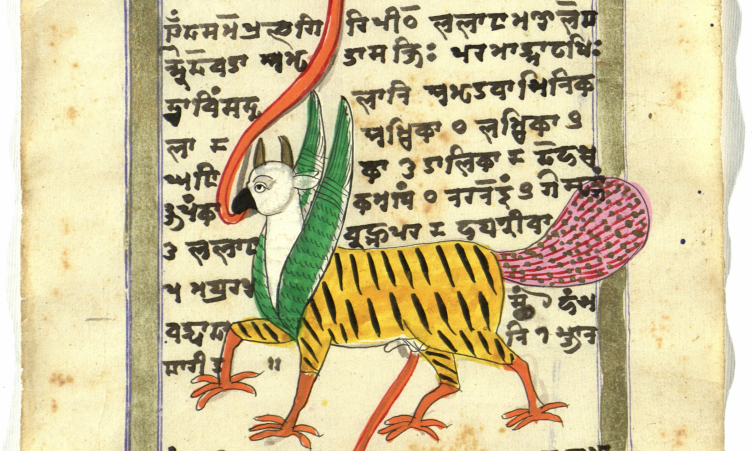
\includegraphics[width=1\textwidth]{pics/Wolpertinger.png}
\caption[The \textit{dehasvarūpa} of \textit{ajapāgāyatrī}]{The \textit{dehasvarūpa} of \textit{ajapāgāyatrī}. The image, reminiscent of a hippogriff, is part of an illustrated Sanskrit manuscript written in the Śāradā script. Preserved as a single large scroll under Acc. No. 1334 at the Oriental Institute in Srinagar (Kashmir), it is entitled \textit{Nāḍīcakra}. The manuscript contains a depiction of the yogic body’s \textit{cakra}s and \textit{nāḍī}s. The text surrounding the figure closely corresponds to the additional material found in manuscript \getsiglum{U2} of the \textit{Yogatattvabindu}. The manuscript reads (diplomatic transcription): \textit{oṃ daśame pūrṇagiripīṭhe lalāṭamaṇḍale candro devatā amṛtāśaktiḥ paramātmā ṛṣiḥ dvāviṃśaddalāni amṛtavāsinikalā 4: ambikā 1 lambikā 2 gha(ṃ)ṭkā 3 tālikā 4 dehasvarūpaṃ kākamukhaṃ 1 naranetraṃ 2 gośṛṅgaṃ 3 lalāṭabrahmapara 4 hayagrīvā 5 mayūramuśchaṃ 6 haṃsacārītani 7 sthāna.}}
	\phantomsection\label{fig_wolpertinger}
      \end{figure}

      \clearpage

  \begin{figure}[ht]
	\centering
  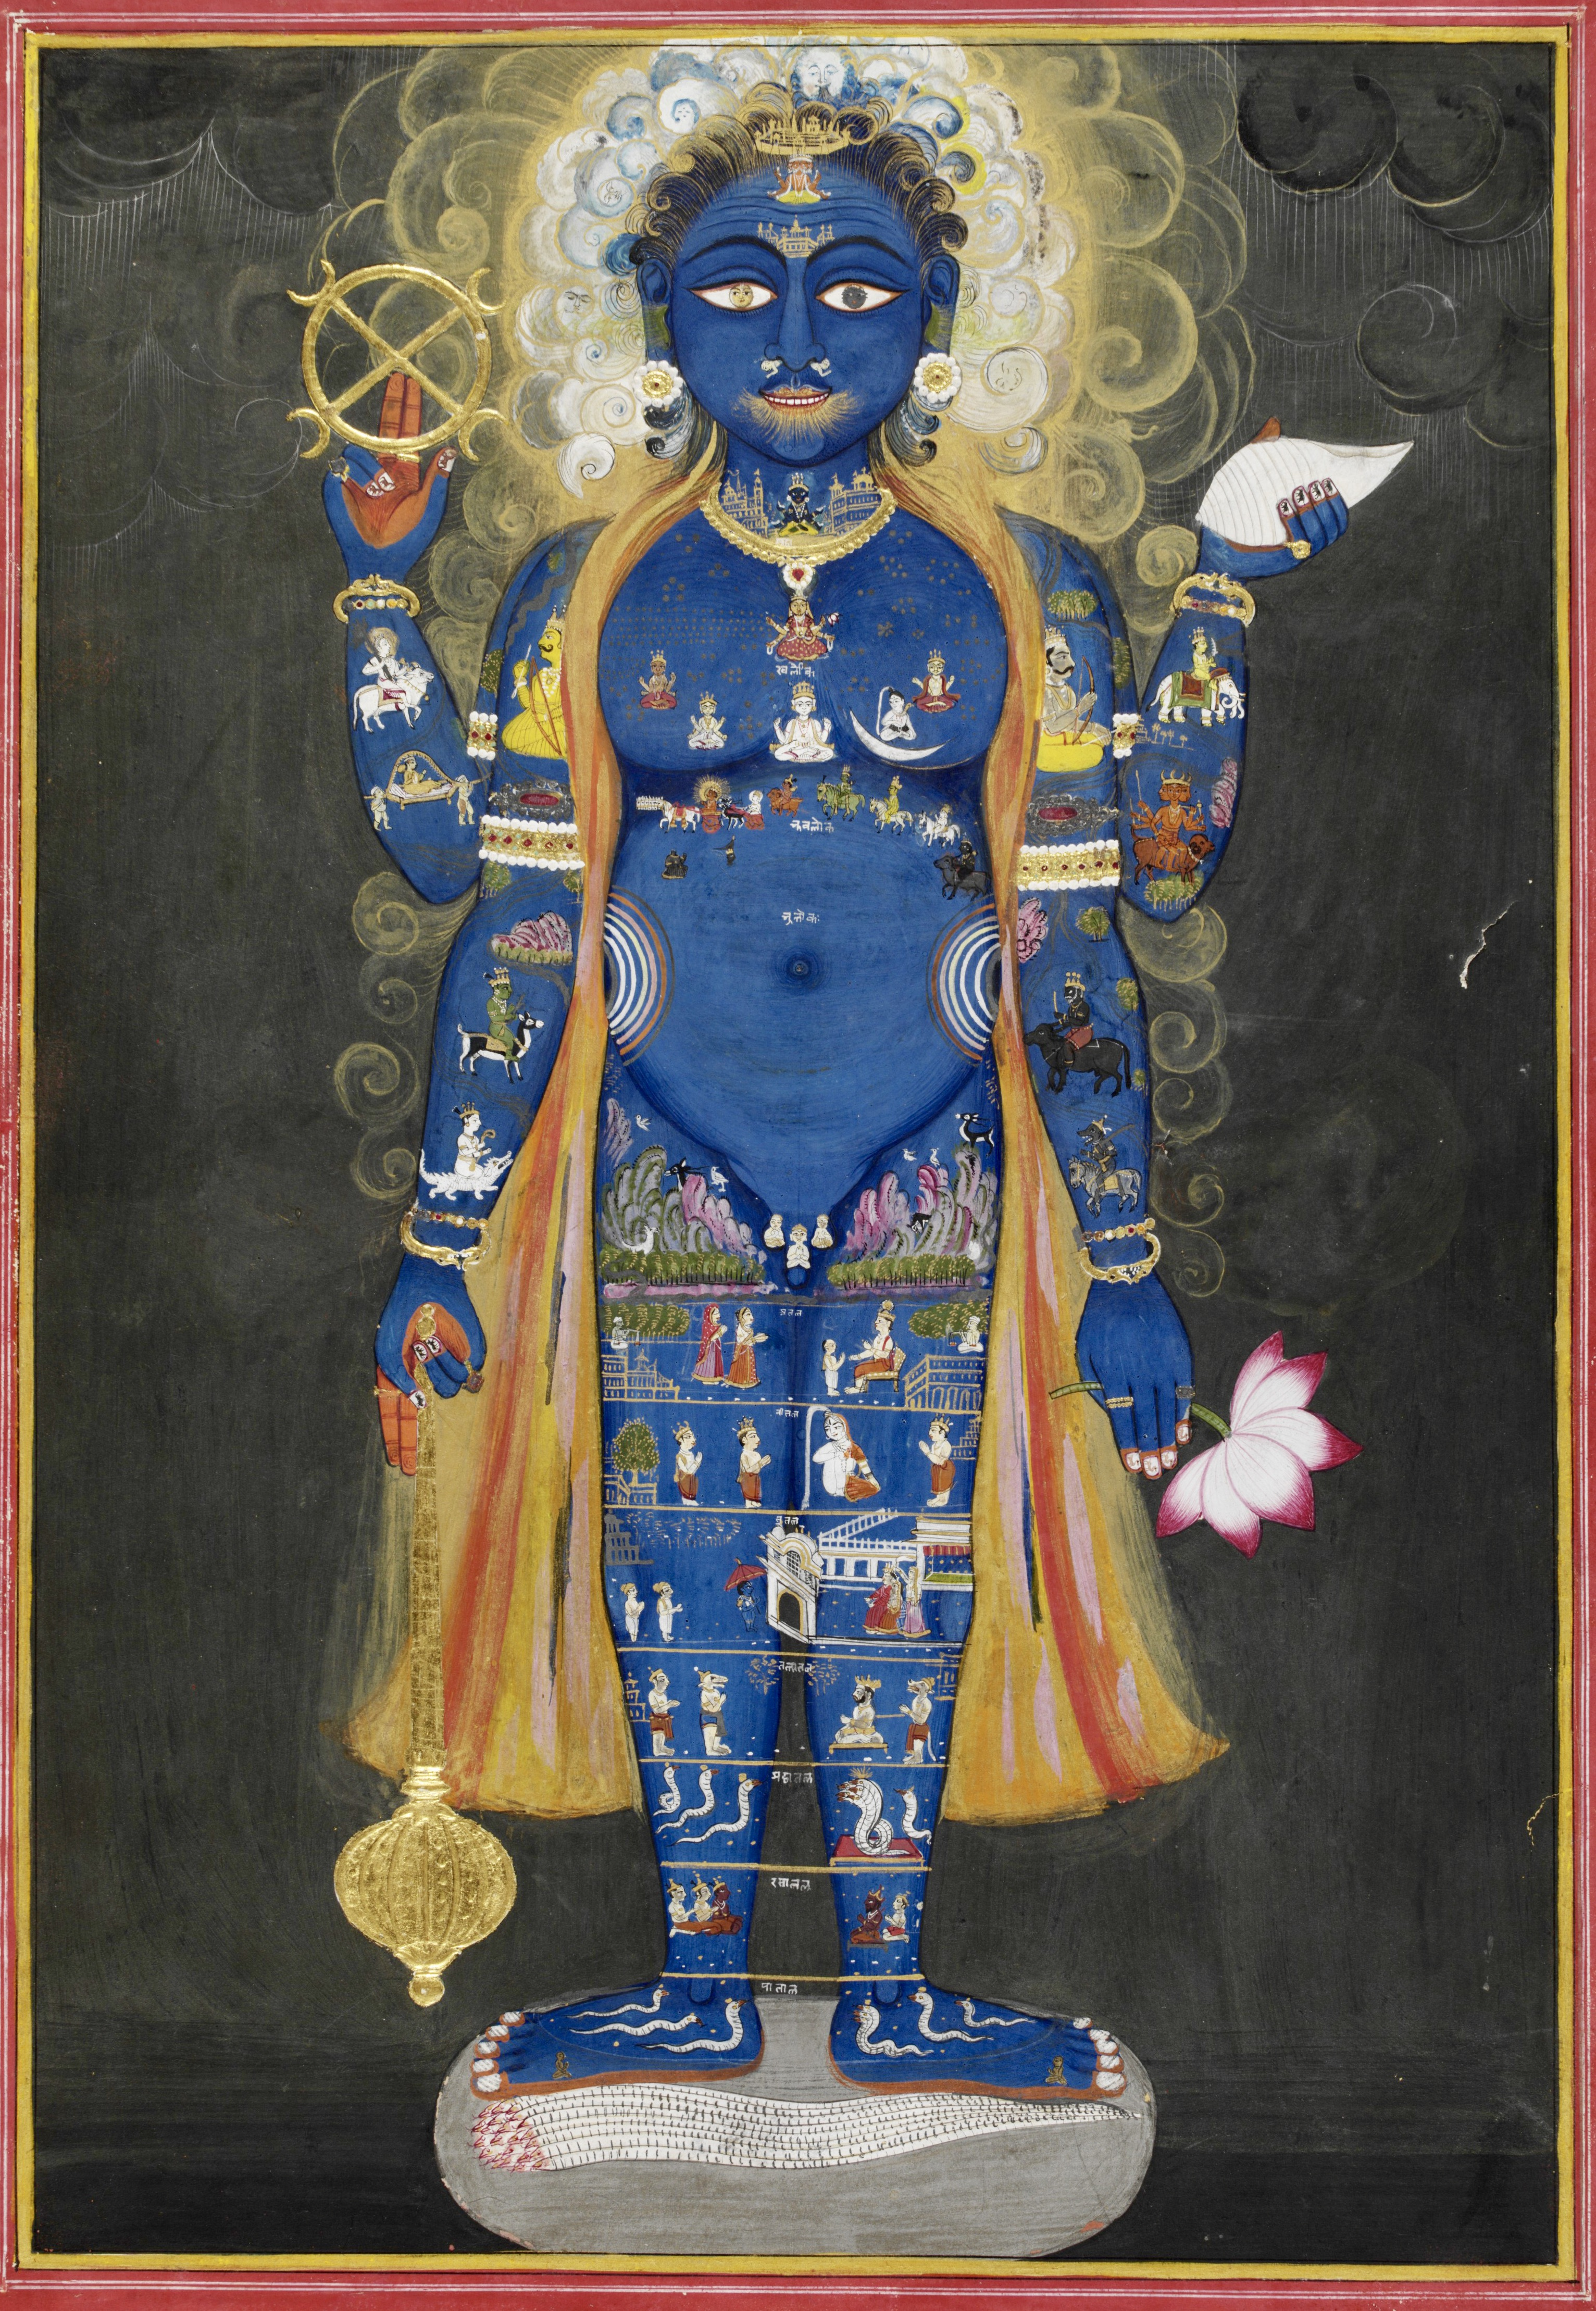
\includegraphics[width=1\textwidth]{pics/Vishnu_Vishvarupa_cropped.jpg}
	\caption{Viṣṇu Viśvarūpa, India, Rajasthan, Jaipur, ca. 1800–1820, Opaque watercolor and gold on paper, 38.5 × 28 cm, Victoria and Albert Museum, London, Given by Mrs. Gerald Clark.}
	\label{fig1}
      \end{figure}
\clearpage
  \begin{figure}[ht]
	\centering
  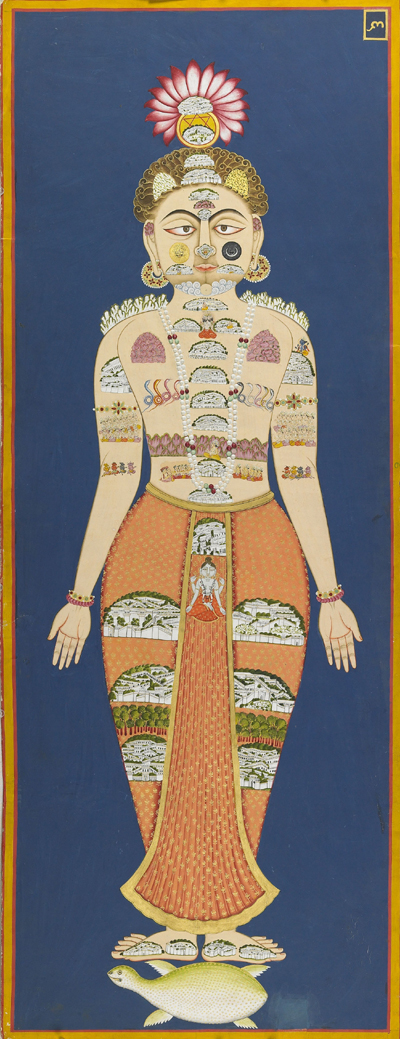
\includegraphics[width=0.5\textwidth]{pics/The_Equivalence_of_Self_and_Universe_(detail),_folio_6_from_the_Siddha_Siddhanta_Paddhati,_(Bulaki),_1824_(Samvat_1881);_122_x_46_cm._Mehrangarh_Museum_Trust..jpg}
	\caption{The Equivalence of Self and Universe (detail), folio 6 from the \textit{Siddhasiddhāntapaddhati} (Bulaki), India, Rajasthan, Jodhpur, 1824 (Samvat 1881), 122 x 46 cm, RJS 2378, Mehragarh Museum Trust.}
	\label{fig2}
      \end{figure}
      % \end{landscape}


\chapter{Bibliography}
 \label{sec:bibli}
\clearpage
\newpage 
\thispagestyle{empty}
\quad  \addtocounter{page}{-1}

\newrefcontext[sorting=tixel]
\printbibliography[heading=subbibintoc, title=Primary Sources, keyword=primary]

\newrefcontext[sorting=nyt]
\printbibliography[heading=subbibintoc, title=Secondary Literature, keyword=seclit]

\printbibliography[heading=subbibintoc, title=Catalogues, keyword=catalogues]

\printbibliography[heading=subbibintoc, title=Online Sources, keyword=onlinesource]

\end{document}
